% This document provides the style to be used for a MSc Thesis at the
% Parallel and Distributed Systems group
\documentclass[11pt,twoside,a4paper,openright]{report}

% use babel for proper hyphenation
\usepackage[british]{babel}
% Graphics: like the DUT logo on the front cover
\usepackage[dvips]{graphicx}
%Enables [H] for figures.
\usepackage{float}
% FONT: times
\usepackage{times}
% for url's use "\url{http://www.google.com/}"
\usepackage{url}
% To allow margin adjustments
\usepackage{changepage}
% To allow listings.
\usepackage{listings}
% To inserts to do's
\usepackage{todonotes}

\begin{document}

%%%%%%%%%%%%%%%%%%%%%%%%%%%%%%%%%%%%%%%%%%%%%%%%%%%%%%%%%%%%%%%%%%%%%%%%%%%%%%%
\hoffset=1.63cm
\oddsidemargin=0in
\evensidemargin=0in
\textwidth=5in

%%%%%%%%%%%%%%%%%%%%%%%%%%%%%%%%%%%%%%%%%%%%%%%%%%%%%%%%%%%%%%%%%%%%%%%%%%%%%%%
\parindent=1em

\pagestyle{empty}

% FRONTCOVER
\begin{titlepage}

\null\vfill

\begin{center}
\LARGE{MultiChain:\\
       		an incremental step in a new distributed data structure}
\end{center}

\vspace{1.5cm}

\begin{center}
Steffan D. Norberhuis\\
steffan@norberhuis.nl
\end{center}

\vfill

\begin{figure}[!b]
\centering

\includegraphics[width={0.5\textwidth}]{pics/TUD_logo_color.eps}
\end{figure}

\vspace{2.0cm}

\end{titlepage}


% EMPTY PAGE
\cleardoublepage

\pagestyle{plain}

% TITLE PAGE: page i (hidden)
\begin{titlepage}

  \begin{center}
  \null\vfill
    \begin{center}
    \LARGE{MultiChain:\\
		an incremental step in a new distributed data structure}
    \end{center}

    \vspace{3cm}

    \begin{large}
    Master's Thesis in Computer Science
    \end{large}

    \vspace{1.5cm}

    \begin{normalsize}
    Parallel and Distributed Systems group\\
    Faculty of Electrical Engineering, Mathematics, and Computer Science\\
    Delft University of Technology
    \end{normalsize}

    \vspace{2.0cm}

    \begin{normalsize}
    Steffan D. Norberhuis
    \end{normalsize}

    \vspace{1.0cm}

    % <MM> DD, YYYY
    \today            %TODO: #36 Dit is de datum van uitgifte van final versie aan de afstudeer commissie

  \vfill
  \end{center}

\end{titlepage}



% GRADUATION DATA AND ABSTRACT: pages ii and iii (hidden)
%De aankondiging bevat de spreker, titel, plaats, datum en tijd, samenstelling van de afstudeercommissie en een korte samenvatting (maximaal 25 regels).
\thispagestyle{empty}

\noindent \textbf{Author}\\
\begin{tabular}{l}
Steffan D. Norberhuis\\
\\
\end{tabular}\\
\noindent \textbf{Title}\\
\begin{tabular}{l}
MultiChain: a cybercurrency for cooperation\\
\\
\end{tabular}\\
\noindent \textbf{MSc presentation}\\
\begin{tabular}{l}
% <MM> DD, YYYY (like \today)
December 14, 2015
\\
\end{tabular}

\vspace{1.1cm}

\noindent \textbf{Graduation Committee}\\
\begin{tabular}{ll}
% The order of listing the names: Graduation prof, supervisor(s), others ordered by title + alphabetical
%examples:
%prof. dr. ir. H. J. Sips (chair) & Delft University of Technology \\
%ir. dr. D. H. J. Epema           & Delft University of Technology \\
dr. ir. J. A. Pouwelse          & Delft University of Technology \\
dr. A. Iosup                    & Delft University of Technology \\
dr. ir. Z. Erkin                & Delft University of Technology \\

\end{tabular}

\begin{abstract} %de abstract bevat alleen een korte samenvatting van de inhoud van het onderzoek
Peer-to-peer networks are often large, collaborative networks where peers can join openly.
The essence of a collaborative, distributed system is that every node performs tasks for other nodes.
The peers help often in singular interactions and without direct reciprocity.
This allows malicious peers to abuse and freeride public goods.
The network without countermeasures can fall into a tragedy of the commons
where no one helps another and everyone takes advantage of the generosity of peers.
Only when the reputation of a peer is publicly available at scale and peers trust this reputation
can the network escape the problems of free riding and attain high utility for all participants.

This thesis focuses on designing and implementing the first step of a tamper proof reputation system within Tribler.
Tribler is a peer-to-peer BitTorrent system developed at the Delft University of Technology.
This first step, made by this thesis, is to create MultiChain, a proof-of-concept bookkeeping system.
MultiChain tracks the upload and download amounts of peers to eliminate free riding.
MultiChain is cryptographically protected and validated.
The bookkeeping system has to be scalable to be publicly available and be able to process enough transactions.
The system has to work in an asynchronous network.

A new design of a distributed data structure that can be used as a ledger is introduced by this thesis.
This first step with MultiChain is already more resilient to tampering than previous work, like BarterCast.
BarterCast had no security measures against tampering records.
Peers are participants of a peer-to-peer network.
The design of MultiChain is to have a chain of blocks for every peer as a ledger.
A block contains a transaction between a peer.
This block is shared and added to both chains.
This makes both chains of the peers intertwined and entangled at a shared block.
The proposed design abandons the typical global, full ledger.
The protocol of creating these blocks between peers is described.
The problems faced by MultiChain in an asynchronous network are explained.
The thesis proposes how the design can overcome these problems
by only allowing atomic operations to be performed on the chain
and to introduce unfinished blocks in the chain.

The implementation of the design is tested and experimented with within this thesis to validate it to work correctly.
Furthermore, a number of weak points are discussed.
These weak points have to be addressed in the future to create a tamper proof reputation system.



\end{abstract}

\clearpage



\pagenumbering{roman}
\setcounter{page}{4}

% EMPTY PAGE: page iv
\cleardoublepage

% OPTIONAL QUOTATION: page v
%\pagestyle{empty}

\null\vfill

\begin{center}
\emph{``TODO QUOTE''} -- TODO QUOTED PERSON
\end{center}

\vspace{10cm}

\clearpage


% EMPTY PAGE: page vi
%\cleardoublepage

% PREFACE: page v
\chapter*{Preface}
\addcontentsline{toc}{chapter}{Preface}
The huge increase in Bitcoin adoption, 
due to the increase in uncertainty in the security of traditional currency 
after the financial crisis in 2008, 
is only rivaled by the speculation of the enormous possibilities 
of the underlying technology of the block chain.
The block chain is the first technology, seen with real world adoption,
that allows to register transactions without a trusted third party.
But the block chain has several limitations in scalabillity 
that will limit Bitcoins in fully replacing traditional currencies with a digital currency.
It also limits block chain as a scalable basis for a large scale reputation system, 
similar to a digital currency, with vast amounts of transactions.
These developments provides motivation to research the properties and possibilities of a variant of the block chain:
MultiChain.

\vspace{1\baselineskip}

\noindent
I would like to acknowledge several people that helped me during my master thesis.
First I would to heartily thank dr.ir. Johan Pouwelse for his mentoring and helping me in setting goals and achieving these goals.
Furthermore I would like to thank dr.ir. Cor-Paul Bezemer for his guidance and help with implementing within Tribler. 
I also would like to thank Elric Milon and Lipu Fei for answering countless questions
and problems I encountered during the programming phase of my thesis.
For the excellent feedback and help to improve my code I would like to thank dr.ir. Niels Zeilemaker.
His support by adding functionality to Dispersy was also invaluable.
Rob Ruigrok was doing his master thesis at the same time
and helped me to avoid problems he encountered before I experienced them as well and
I am grateful for this help.
I am also very thankful for the companionship I felt within my work room 
and I would like to thank especially Hans Bogerts BSc, Niels Doekeijmeier BSc and Ernst van der Hoeven BSc.
You certainly made my work more enjoyable.

\vspace{1\baselineskip}

\noindent
Steffan Derk Norberhuis

\vspace{1\baselineskip}

\noindent
Delft, The Netherlands

\noindent
\today

% EMPTY PAGE: page vi
\cleardoublepage

% TABLE OF CONTENTS: starting at page vii
\setcounter{tocdepth}{1}
\tableofcontents

\cleardoublepage

\pagenumbering{arabic}
\setcounter{page}{1}




% CHAPTERS ... For instance: History/Prior Work, Design/Implementation, Experiments
% INTRODUCTION
\chapter{Introduction}
\label{chp:introduction}
Tribler is a peer-to-peer file sharing program developed by the Delft University of Technology for research purposes.
Tribler expands the BitTorrent protocol and has added multiple improvements on this protocol.
The main focus of Tribler is to make security and privacy the default for Internet users and impossible to shutdown.
A fully distributed program, not relying on any central component, is needed to achieve this.
Tribler has been designed and build using this methodology\cite{Pouwelse-tribler}\cite{Bakker-tribler}.
This master thesis was conducted as part of the research mission to improve Tribler.

\vspace{1\baselineskip}

\noindent
TODO ORGANISATIONAL DESCRIPTION OF THESIS

\section{Tribler}
%TODO update
In peer-to-peer file sharing a node called a seeder uploads parts
of a file to another node, the downloader.
The role of being a seeder and downloader constantly changes
and a node can be both at the same time for different, parallel connections.
A seeder can become a downloader when they wish to download other files
and downloaders can become seeders,
if they posses a file someone else wants.
The ratio between the total size downloaded and uploaded is called the seeding ratio\cite{Cohen-bittorrent}.
private community source

The uploading can be seen as an interaction of one node helping another node.
These interactions comes at the cost of consuming bandwidth for both parties.
There is only direct benefit for the downloader.
The downloader receives a file he wants.
There is no direct barter between the seeder and downloader.
As the seeder does not get anything in return for uploading the file.
Although it can happen by chance that a downloader is also a seeder directly to the original seeder,
but this is unlikely\cite{Lai-Incentives}.

If everyone contributes, files become more available and are downloaded at higher speed.
This claim is supported by measurements taken in private communities
\cite{meulpolder-privatecommunities}.
In private communities high seeding ratio's are enforced by a third party.
Both high availability and high download speeds result in a higher utility for the downloaders.
But currently freeriding in these networks takes places in high quantities\cite{Adar-Freeriding},
The BitTorrent Tit-for-Tat protocol is not enough to stop abuse\cite{Pouwelse-tribler}.

Tribler wants to achieve a high global seeding ratio by making it benificial to have such a ratio.
Nodes can award each other with higher cooperation if a node has a reputation itself to be cooperative.
This requires for a tamper-proof interaction history to base a reputation on in a network.
Those contributing more receive more help in return,
and malicious nodes cannot abuse the network by tampering with the interaction history.

Tribler has recently implemented anonymous connections using onion routing.
This feature allows downloaders to become indistinguishable from other users in the network.
But every data packets has to be forwarded
by a number of intermediate hop between the downloader and seeder\cite{Plak-anonymous}.
The requirement of forwarding packets increases the network load of data being sent.
The total cost of bandwidth per file is increased,
but also the number of nodes helping a single node downloading a file increases.
This in turn increases the necessity of an incentive system to reward collaboration.


%Problem description
\chapter{Problem Description}
In a distributed system nodes will have interactions with other peer nodes.
A node will have to decide how to react to these peers.
Our work is beneficial to the process of deciding how to react to these peers.

In this chapter the problem will be described of how to decide to react to a peer.
The problem will first be explained in a simplified form.
Using this simplification, the problem will be transformed gradually
to the real world problem faced in distributed systems today.
Finally several real world examples of the problem will be described.

\section{Deciding to help}
Nodes can decide to cooperate with a peer or decide not to help a peer and defect.
This is the traditional Prisoner's Dilemma 
and we will explain this dilemma\cite{Nowak-PrisonerDilemma}\cite{Lai-Incentives}.
Nodes can help each other at a cost, a negative utility, 
but the recipient of the help will receive a beneficial utility from the help.
The benefit received is greater than the cost and is denoted by $R$ for reward.
But if one node chooses to not help the other node,
 then he will still receive a beneficial utility and at no cost, $T$ for temptation.
The node that provided the aid will now receive no benefit and only incur a cost $C$.
If both nodes choose to not help each other, 
then they will both receive a penalty $P$, which is higher then the cost of helping each other.

This dilemma can be repeated several times with the same nodes and is the Iterated Prisoner's Dilemma.
Each time both nodes will have to decide if it will help the other node.
The utility received can be seen in Table \ref{tab:pd-um}.

\begin{table}[h]
\center
	\begin{tabular}{l|ll}
	A\textbackslash B       & cooperate  & defect     \\ \hline
	cooperate & $R_A /R_B$ & $T_A /C_B$ \\
	defect    & $T_A /C_B$ & $P_A /P_B$
	\end{tabular}
\caption{Prisoner's Dilemma utility matrix}
\label{tab:pd-um}
\end{table}

A rational node wants to receive maximum benefit at a minimal cost.
The node will follow a strategy that he believes will achieve this.
At first it might seem that a node will always choose to defect,
because it will never incur a cost and receive maximal benefit.
But the other node will be reluctant to help a node if the aid is never returned.
Simple strategies, like tit-for-tat or win-stay, lose-shift, suffice in the Iterated Prisoner's Dilemma
and will perform well\cite{Nowak-Cooperation}.

In a large scale, distributed system, this dilemma occurs with every interaction between nodes.
The node can already be familiar with the peer,
but more often the peer will be a peer the node has not interacted with before.
A further complication is that help is one way and can no longer be exchanged.
This complication excludes the direct opportunity to barter for help 
or to barter for help in the future\cite{Lai-Incentives}.
The performance of the tit-for-tat or win-stay, lose-shift strategies
quickly deteriorate in such a situation.

For a node it is easier to abuse the generosity of others in this more anonymous situation.
Nodes that help others will be penalized through the cost they incur
and incentivized to adopt the malicious behavior themselves.
Nodes in general will become more reluctant to help nodes\cite{Nowak-PrisonerDilemma}.
In the end no node will help another and all nodes will receive a penalty.
This is commonly called the Tragedy of the Commons in the literature \cite{hardin-tragedy}.
The whole network will actually receive more benefit in total if everyone would corporates.
But nodes have no way of knowing if the peer they meet are willing to help.

\section{History of decisions}

In the Iterated Prisoner's Dilemma the history of the previous transactions can be used 
to see if a node helped others in the past.
The simple strategies, previously mentioned, use a history to improve performance
to avoid getting abused.
But this private history is not effective to achieve high overall utility in distributed systems,
because the peers are often interacted with for the first time.
No history is known for these peers.
A public history of node, containing every previous interaction, is necessary to prevent abuse
and is able to achieve high overall utility\cite{Lai-Incentives}.

A history can be used to create a currency or a reputation system.
The node providing help will receive a boost in currency or a beneficial reputation.
The currency or reputation can be used in the future to receive aid.
In a currency system, receiving help will transfer currency to the helper.
In a reputation system, only nodes with a sufficiently good reputation will be helped.

The currency or reputation has to be made publicly available to all nodes in the network.
But a node publicizing to hold a certain reputation is not sufficient as it is not trustworthy.
So a interaction history, that contains every prior interaction a node has conducted, is publicized.
Nodes can cross-reference the interaction history with other nodes and calculate the amount of currency 
or the reputation that a node has.
Based upon this calculation, the node can decide to provide aid or not.

The interaction history has to be distributed among the nodes in the network
to become publicly available.
Efficient distribution protocols are a difficult challenge themselves and outside the problem scope.
But distribution is worth mentioning, because it puts constraints on the interaction history.
The interaction history has to be distributable in an efficient manner.
Only if it meets these constraints, will an interaction history be usable in a distributed system.

\section{Tamper-proof to facilitate thrust}

Interaction histories only prevent direct abuse of the generosity of the nodes.
A malicious node can still try to tamper with the interaction history.
An example of a type of these attacks are double spending attacks\cite{Nakamoto-bitcoin},
where a interaction is altered.
But a node can also try to deny an interaction.
The interaction history has to be resilient to attacks that tamper the interaction history, 
or no one will trust the history.

A digital currency system builds upon trust just as much as a banknote currency.
A reputation system will also need a level of trust.
A system cannot be fully secure, 
but still a reasonable certainty can be achieved that no tampering of the interaction history can occur.
Reasonable certainty is for example that no attack can happen 
if more than half of the network consists of honest nodes.

\section{Real world examples}
In this section we will describe real world problems of the problem type introduced.
This is meant as an illustration of the real world problems and is not a complete survey.

Ad hoc networks are networks that rely on the willingness of nodes to cooperate
and forward messages to each other.
These messages are forwarded at a cost to the node.
For example, the cost can be the power consumption, 
which is limited due to the node running on battery power.
Energy efficiency becomes a prime concern for these node. 
Every node may not display the same willingness to forward messages and be more selfish.
Protocols that use currency or reputation are already proposed
for this problem\cite{Anderegg-AdHoc}.

In BitTorrent networks nodes help each other to download files by sharing chunks of files.
Especially in these networks are interactions with the same node infrequent\cite{Lai-Incentives}.
Cooperating nodes should receive more aid in the form of higher download speed,
then the nodes that feed upon the network and contribute no upload speed to the network.
It has been shown that in these network
free riding takes place in large quantities\cite{Adar-Freeriding}.

%Related work
\chapter{Related Work}
In this chapter we will discuss related work on tamper-proof interaction histories.

\section{Bitcoin}
Bitcoin is a digital currency that uses a interaction history 
to keep track of transactions made between nodes.
The interaction history is a datastructure called the block chain.

The block chain imposes limits on Bitcoin in several ways.
These limitations on Bitcoin can be seen as the initial motivation for our work.
How Bitcoin uses the block chain technology will be introduced first.
In the following, the limitations imposed by the block chain will be explained.

We will only introduce how Bitcoins uses the block chain and why it does so in such a way.
This section is not a full explanation of the Bitcoin protocol
and only discusses relevant parts of the Bitcoin protocol.
The best starting point for a full explanation of Bitcoins 
is the original paper by Nakamoto\cite{Nakamoto-bitcoin}.
Further information and improvements on Bitcoin can be found on the Bitcoin website\cite{Bitcoin.org-site}.

\subsection{Block Chain}
For a currency to work, people have to be able to trust with a reasonable certainty that no double spending can occur.
Double spending With physical tokens is impossible,
but the same guarantee is not trivial for digital currencies without a trusted third party.
Bitcoin has multiple safe gaurds that work together to prevent double spending.
These safe gaurds will be introduced during the explanation of how Bitcoin works.

The core of the Bitcoin protocol is the block chain.
The block chain contains every transaction of bitcoins.
A transaction consists of three parts.
The first part is the public key the new owner of the bitcoin.
The hash of the whole, previous transaction and the public key of the new owner is concatenated.
This concatenation is hashed and this hash is the second part of the transaction.
The third final part is signature by the current owner of the hash of the concatenation.
The previous transaction is a transaction of the same bitcoin.
The ownership of the bitcoin by the current owner can be verified
by verifying the whole history of the bitcoin.
A transaction is usually shortend to Tx in Bitcoin related work and is used in images in this report.

\begin{figure}[H]
	\centerline{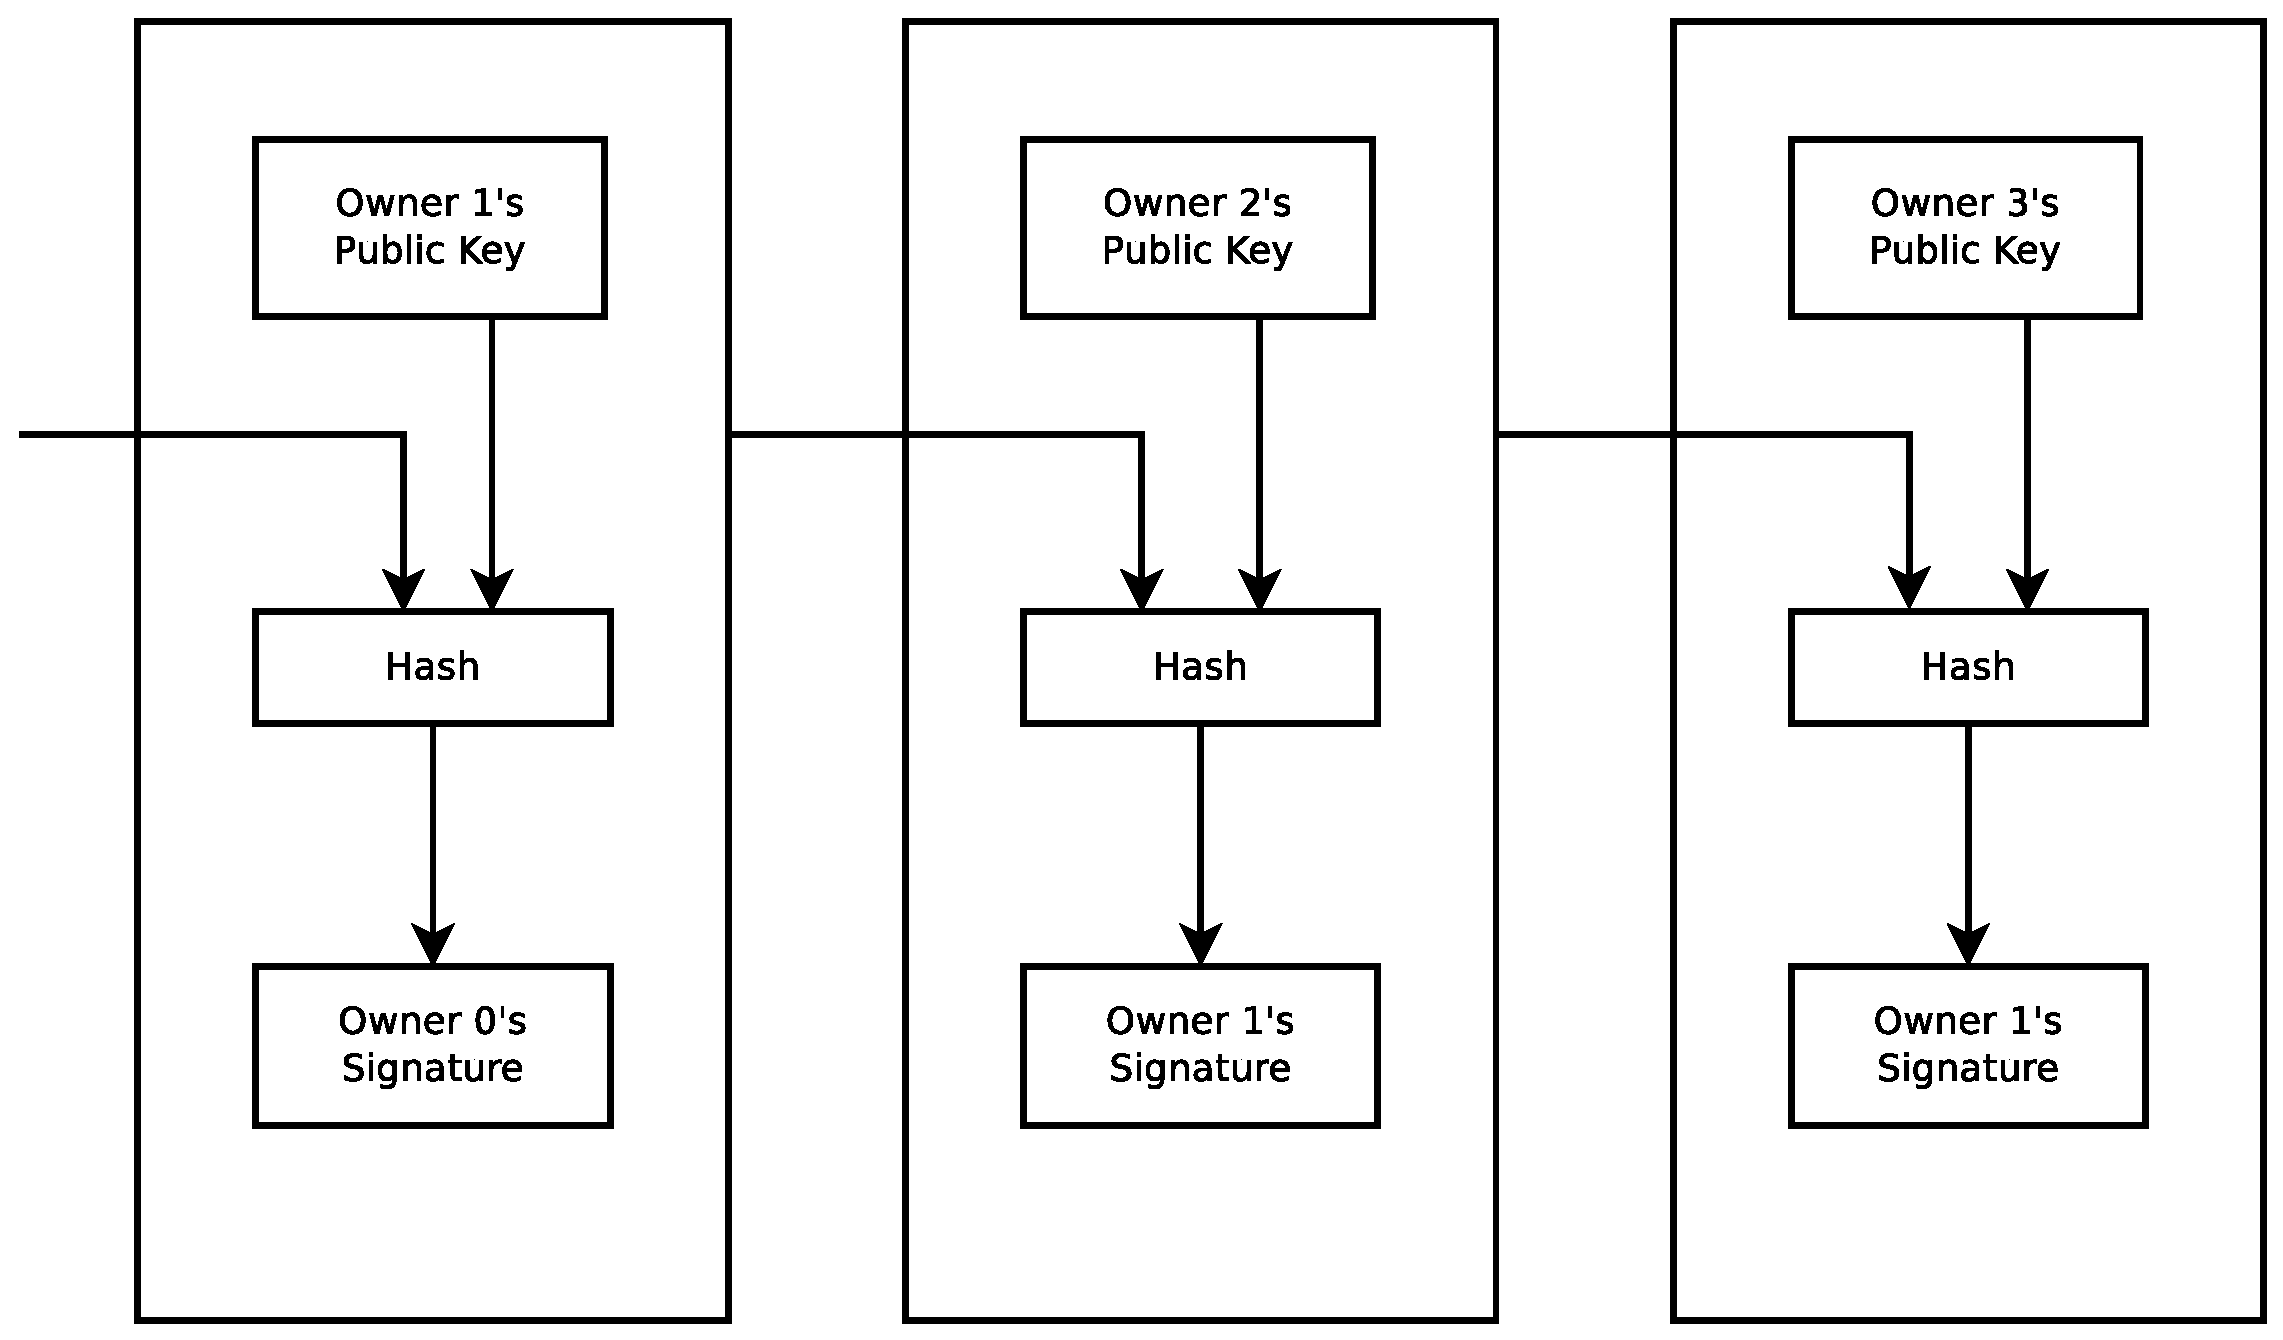
\includegraphics[scale=0.3]{relatedWork/figs/transactions.eps}}
	\caption{Transaction chain}
\end{figure}

Multiple transactions are aggregrated into a single block.
Every block contains the hash of the previous block.
This creates the block chain.
Transaction chains across span several blocks inside the block chain.

These blocks are created by nodes in the network, so called miners.
A miner receives transactions from other nodes in the Bitcoin network.
An attacker can malicously transmit transactions to double spend a bitcoin he owns or does not have.
So every transaction is verified on arrival at a node.
Any transaction that is invalid is just dropped by the node.
No penalty is awarded to the malicous attacker.

The transactions are received in a non deterministic way induced by network characteristics.
The non deterministic nature causes blocks to differ from miner to miner.
The order of transactions has to be agreed upon by the network to eliminate this inconsistency.

Bitcoin uses election to pick the next block  based upon a Proof-Of-Work system.
A nonce is added to every block. 
This nonce is just a number that can be varied,
but is only sound if the hash of the whole block starts with a certain number of zeros.
Miners have to find the correct nonce for their block and this is a proof of work.

\begin{figure}[H]
        \centerline{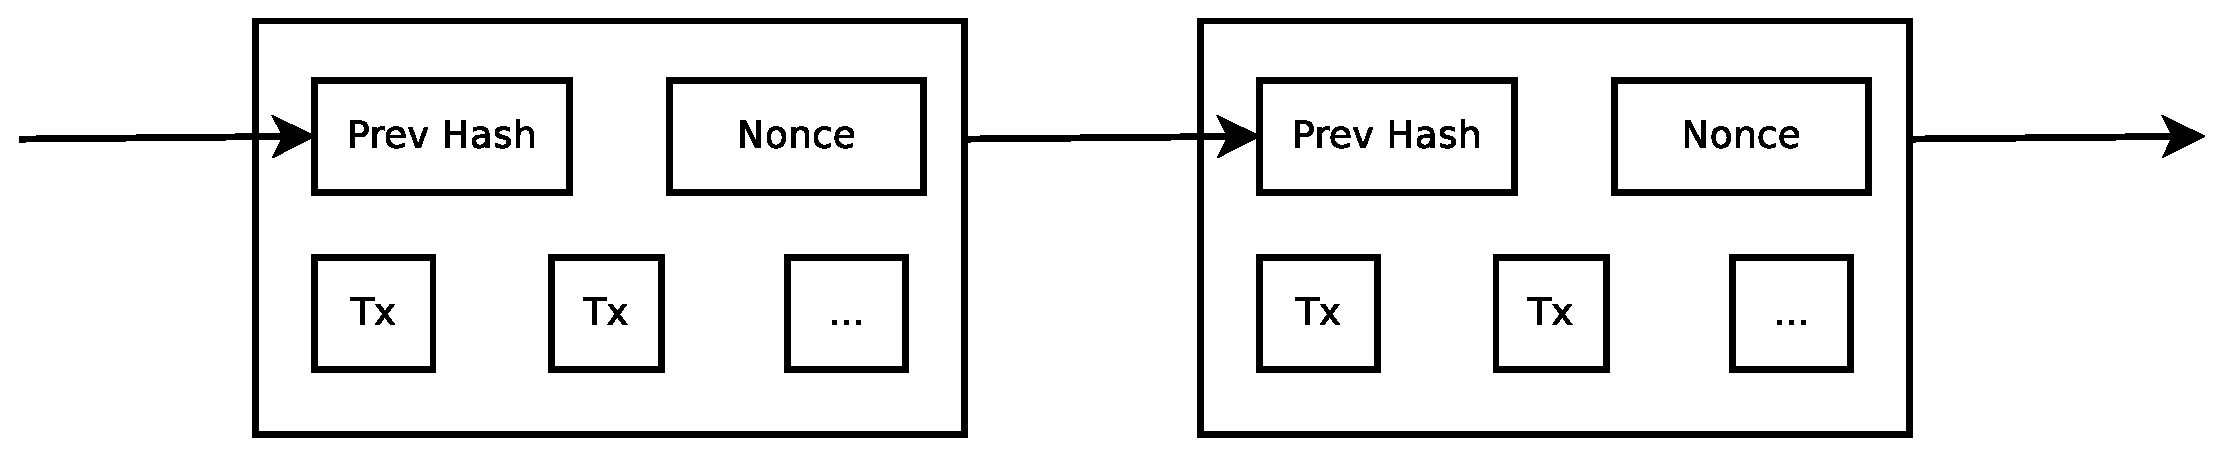
\includegraphics[scale=0.3]{relatedWork/figs/blocks.eps}}
        \caption{Block chain}
\end{figure}

But miners can still find a valid nonce at approximately the same time
and notify parts of the network of their newly found block.
This leaves the network again in an inconsisted state.
These multiple versions of the next block attached to the previous block can be seen as branches.

To solve this inconsistency, Bitcoin nodes save both branches and continue using the longest branch.
At some point one branch will become predominant in the network.
More nodes will dedicate compute power to extend this branch and the growth rate will increase for this branch.
The faster growth rate will ensure that the branch will be adopted by the network as a whole.

The amount of zeros needed in the hash is adjusted to compensate for the fluctuating speed of the network to be able to find nonces.
This is called the hash speed and is the amount of hashes calculated per second.
The hash speed of the Bitcoin network has increased nine fold.
The amount of zeros balances the probability of branches occuring
and the time before a new block is found,
which in turn is how fast transactions are processed.
The growth of the hash speed can be seen in \ref{fig:hash-speed}.

\begin{figure}[H]
        \centerline{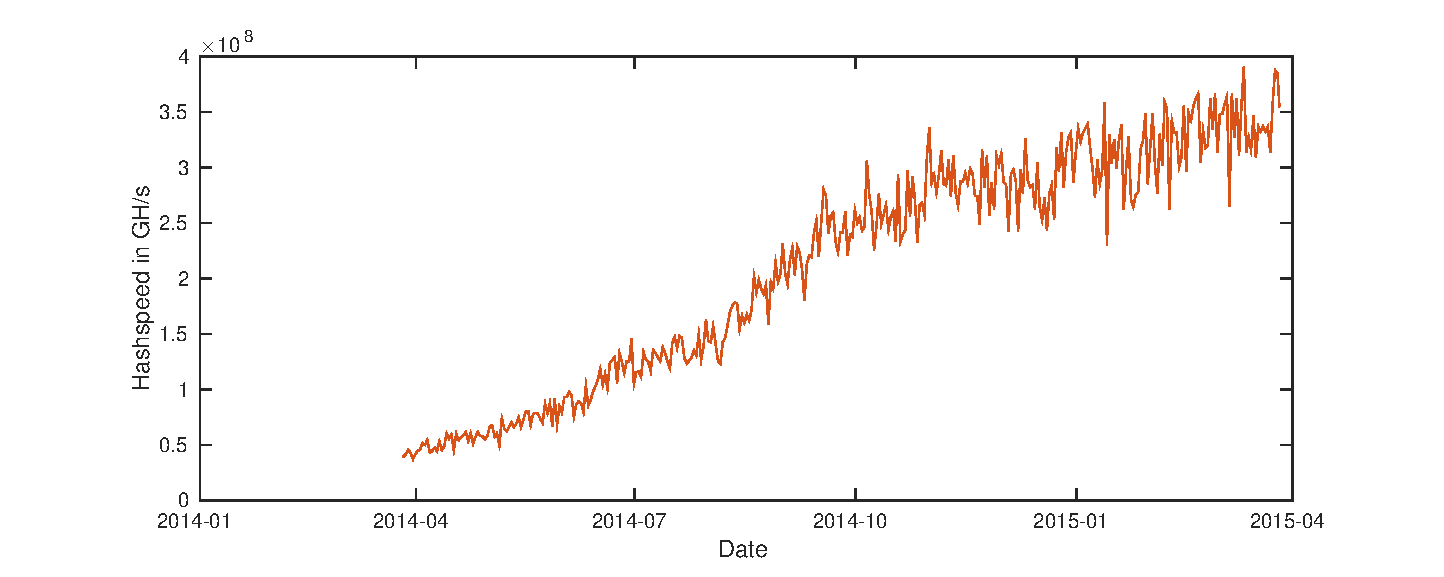
\includegraphics[scale=0.6]{relatedWork/figs/hashspeed/hashspeed.eps}}
        \caption{Amount of hashes calculated per second in the Bitcoin network.\cite{Blockchain.info-bcs}}
	\label{fig:hash-speed}
\end{figure}

Another possible attack to double spend a bitcoin is by sending a transaction to one part of the network,
but to the other part of the network a transaction with a different receipient.
It is possible that both transactions will be introduced into the block chain, but in different branches by two independend miners.
Eventually one branch will win and the attack is averted.

The behaviour just described makes that a transaction can never be confirmed with full certainty.
Another branch could possibly always over take the current longest branch.
This also makes the network vulnerable if the total compute power is owned by a malicous attacker is more than the total compute power of the honest nodes, 
even if the attack has control of 51\% of the compute power. 
In the end the current branch can be overtaken by a new branch started by the attacker.
This new branch allows the whole transaction history to be rewritten by the attacker.
Bitcoin introduces points in the chain that are to be considered final and can no longer change.

\subsection{Limitations}
In this section we will discuss the several limitations of Bitcoins
that originate from the use of the block chain.

\subsubsection{Size}
To be able to prevent double spending and rightfull spending by the right owner, 
the node verifying a transaction needs to be aware of the full history of a bitcoin.
This results in that a node needs the entire block chain to verify a transaction.

The block chain is a data structure ever increasing in size.
No block or data contained in that block is removed.
The block chain has been growing since its inception in 2009.
The size and growth can be seen in figure \ref{fig:bc-size}.

\begin{figure}[H]
        \centerline{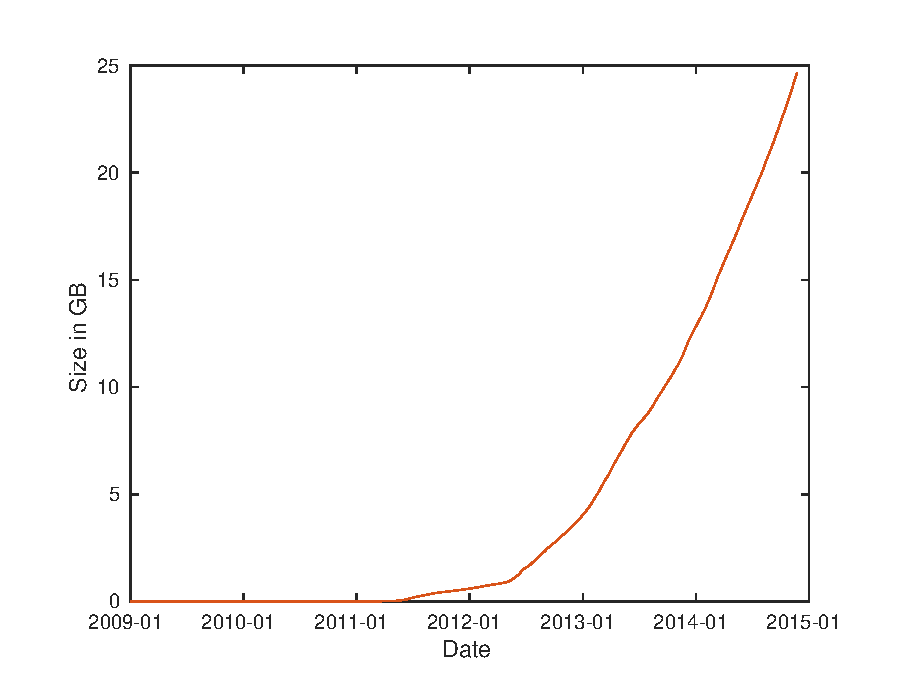
\includegraphics[scale=0.6]{relatedWork/figs/blockchainsize/blockchainsize.eps}}
        \caption{The size of the block chain.\cite{Blockchain.info-bcs}}
	\label{fig:bc-size}
\end{figure}

The size of the block chain at time of writing already prevents less powerfull devices
to operate on the block chain.
This problem is only going to become bigger with the continued creation of transactions
and at a faster pace due to increased adoption of Bitcoin.

This problem was already identified by Nakamoto in his original paper on Bitcoin.
The paper proposes Simplified Payment Verification (SPV).
In SPV mode a node only downloads the block headers of the longest chain.
If a transaction is to be verified, it requests from the network the specific transaction
along with a Merkle tree linking it to a block in the chain.
The Merkle tree can be used to verify that the transaction was included into the block chain.
This allows to calculate with some confidence that the transaction was accepted.

SVP only gives reasonable confidence and is not as secure as running a full node.
Trust has to be placed in the nodes that send the block headers and Merkle Trees.
Secondly, a transaction that is recorded in a more recent block is less difficult to tamper with
than a transaction deep down in the block chain.
This is only an acceptable solution for clients willing to accept more risk due to having a less secure system.
Therefor it is not a solution for the problem for every one.


%Design
\chapter{Design and implementation}

\section{MultiChain Community}
Tribler uses communities to add functionalities to peers.
A peer loads in a community and this community provides a set of messages and endpoints for other peers.
The community can communicate with the endpoints of other peers as well and send a message to these endpoint.
Other peers are automatically discovered using Dispersy.
Examples of a community are the TunnelCommunity that adds functionality to download anonymously\cite{Plak-anonymous}
or the AllChannelCommunity to distribute torrent files.
The designed system will be implemented by adding a new community to Tribler.

The MultiChain community can be run standalone,
but its main use is to integrate with Tribler and track up and download for torrents.
It will replace the current reputation system Bartercast in the future.
\section{Abandoning full transaction history distribution}
One of the main pillars of the design is to have a transaction history for every peer.
This is in contrast to not distribute a common, full transaction history containing the transactions of every peer.
For example used in the design of the blockchain of Bitcoins, discussed in section \ref{sect:bitcoin}.
The reasoning behind the idea to abandon is that a common, full truth
will become the bottleneck in the system.
This will limit the amount of interactions that can be processed
or will limit the participiation of less powerfull machines.

The reason for the limitation is that every interactions will have to be distributed to every peer in the network.
Every transaction has to be processed by every node at the cost of bandwidth, compute power and storage.
The cost might be very limited for a single transaction,
but with greater scale these cost will add up.
The amount of these three resources is limited and will limit the amount of transactions that can be processed.
This problem can be seen to affect Bitcoins and has been demonstrated in section \ref{bitcoin-limit-size}.

Every node has its own transaction history and only needs the transaction history of its peers it interacts with.
The amount of bandwidth, compute power and storage is limited to the minimal needed amount
that is needed to process only the relevant transactions.
This should allow low-powered devices to keep participating when they only have a low volume of transactions.
It also allows higher volumes of transactions in the system as a whole.
\section{Transactions}
A peer will have transactions with other peers in the network.
The peer will want to have an increase in his reputation and have a transaction be created.
The transaction contains the information about how much data was uploaded and downloaded between the peers
and their total upload and download amounts.

The transaction will be encapsulated inside a single block.
A block contains both public keys of the peers,
so it is possible to see between which peers the transaction is.
Both peers sign the block to acknowledge that the transaction has happened.
Every block only contains one transaction.

The blocks are linked to previous blocks by adding the hashes of the previous blocks of both peers.
This creates a directed acyclic graph of blocks.
A chain can be identified within this graph for every peer.
This chain contains every transaction of a peer.

An example of three blocks can be seen in Figure \ref{fig:chain-example}.
The arrows denote the corresponding hash or signature.
In this example the first block is between peer B and C.
The block contains hashes to the previous blocks of both B and C
and can be seen by the outward arrows.
Inside the block it can be seen what part peer B and C signs by the boxes.
The whole block is not signed by both parties.
The reason for this is explained in section \ref{design:block_creation}.

In the example both peer B and C also conduct a transaction with another peer, A and D respectively.
This creates two new blocks and are chained to the block between B and C by adding the previous hash to the new blocks.
The new blocks also contains the previous hashes of A and D
and chain the new block to previous blocks of A and D.

\begin{figure}
	\centerline{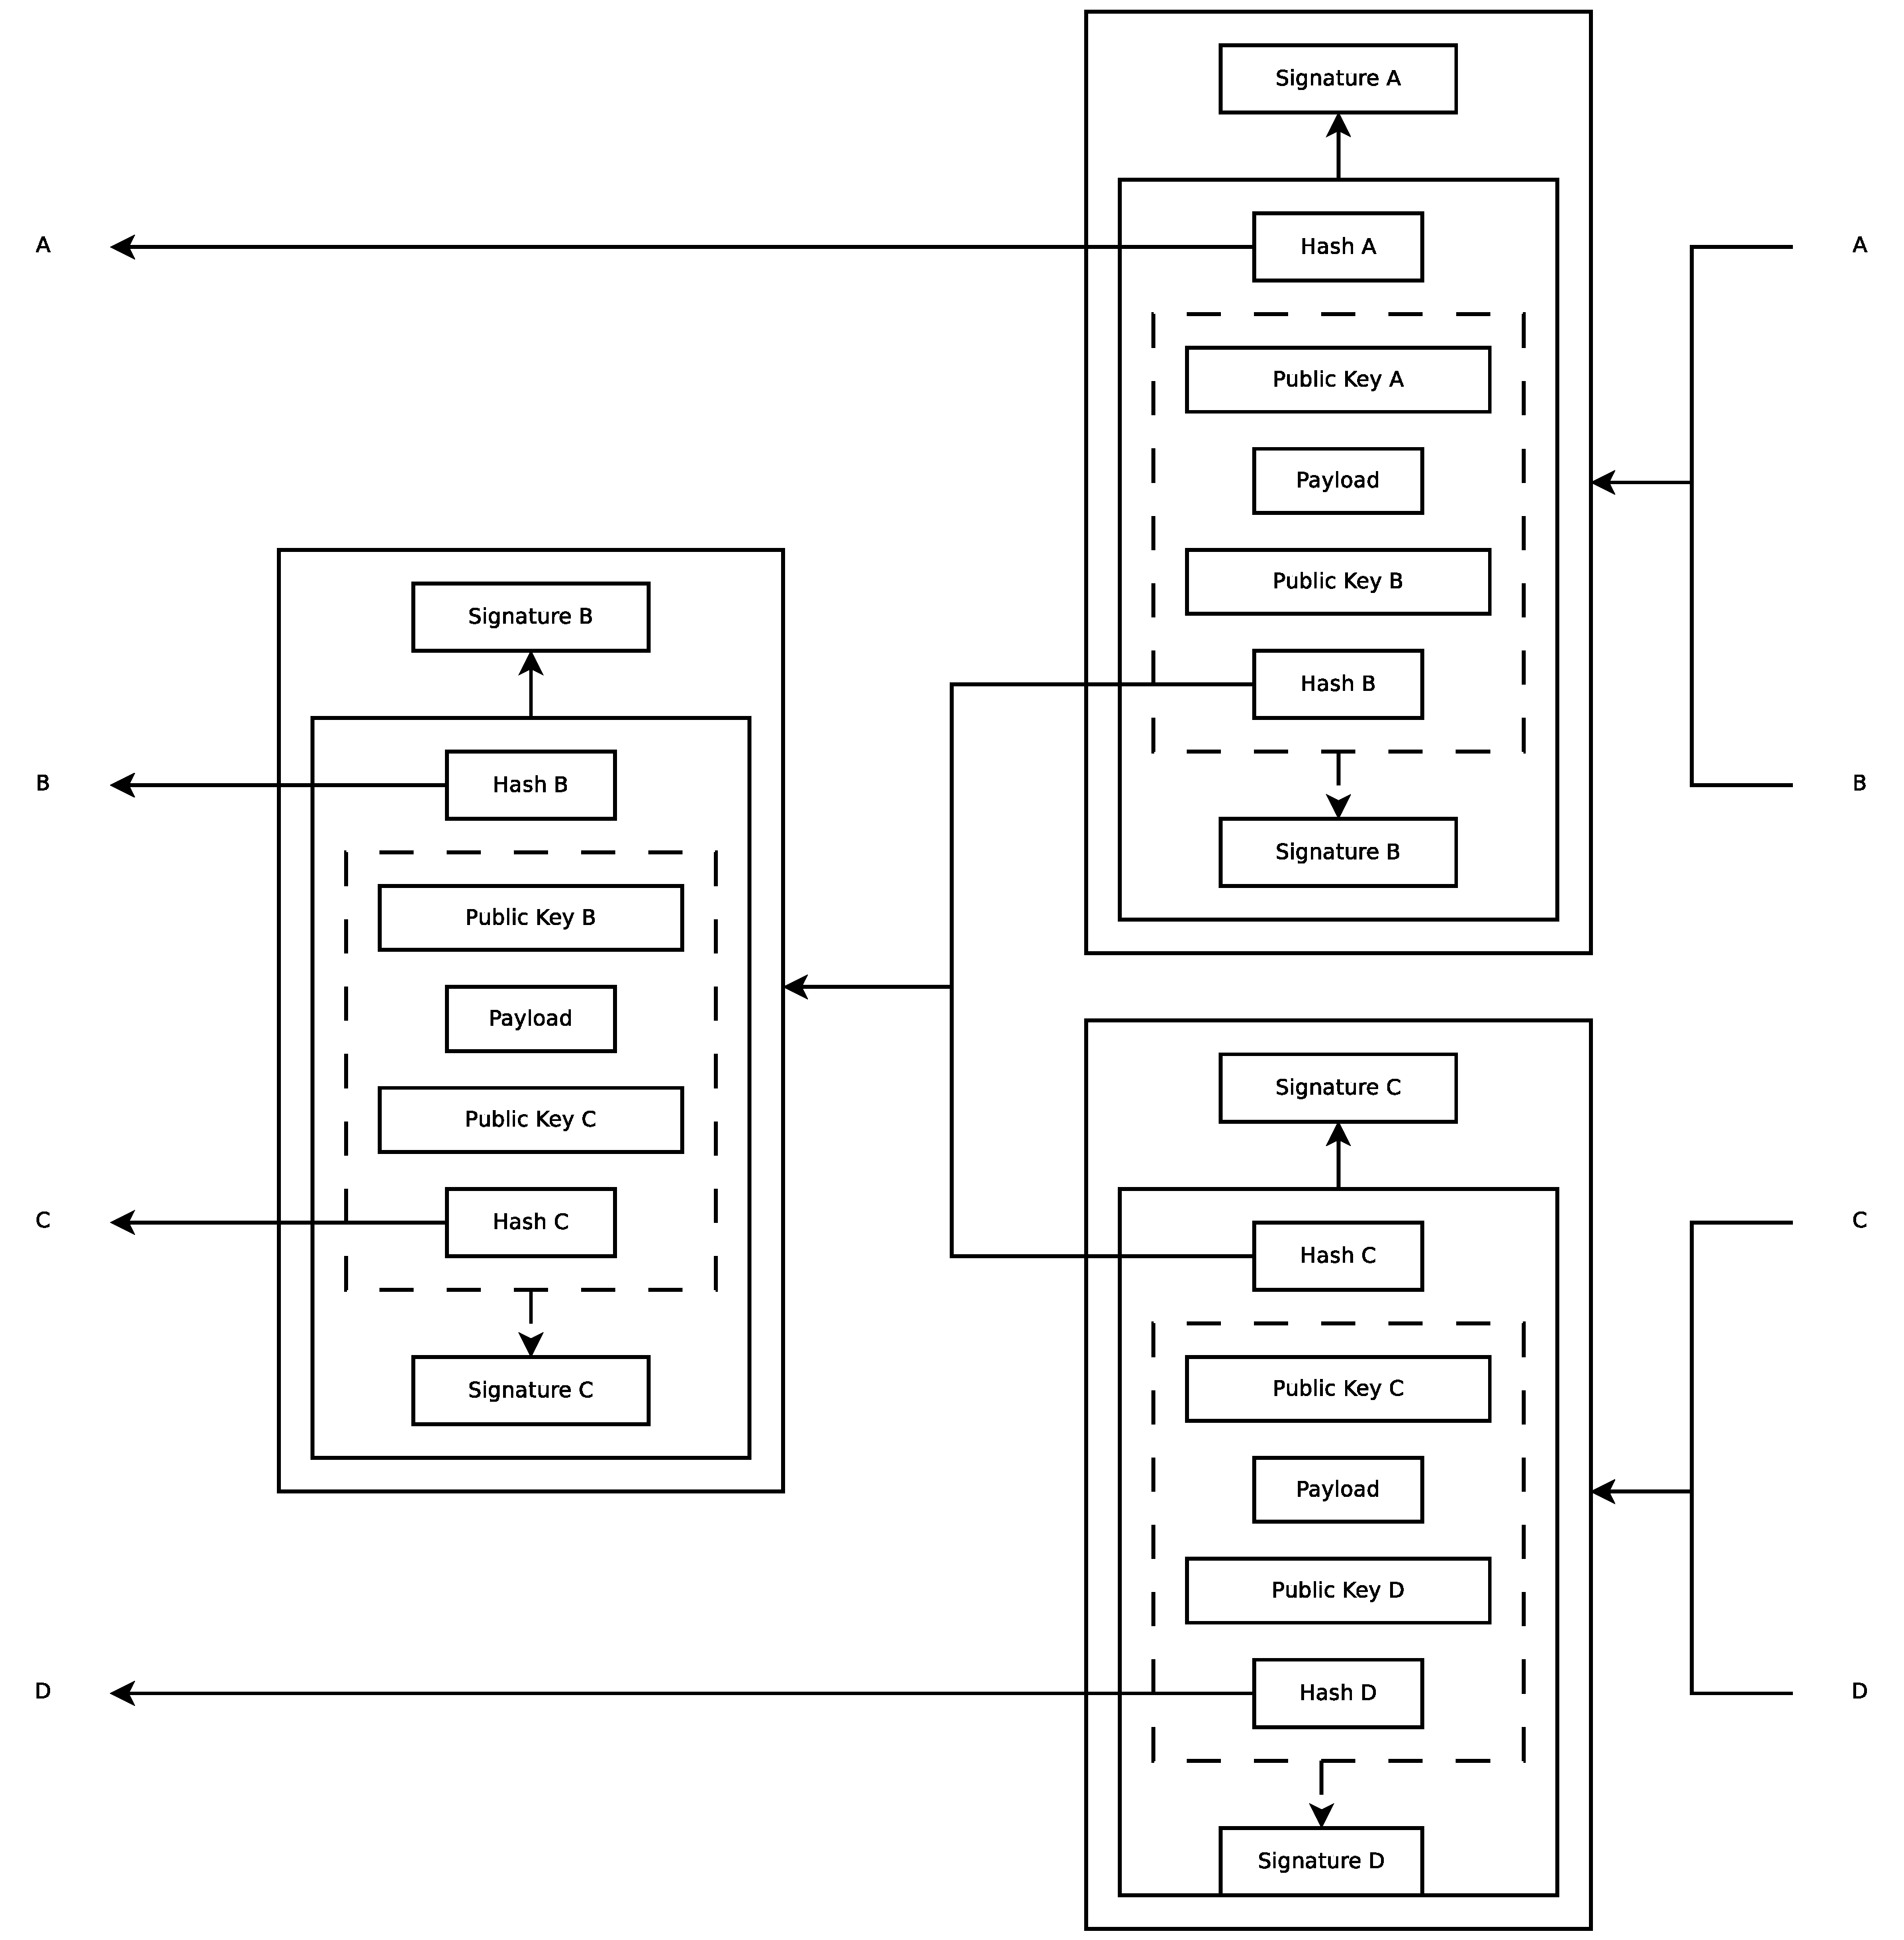
\includegraphics[scale=0.3]{design/figs/chain.eps}}
	\caption{Example of three blocks in the chain.}
	\label{fig:chain-example}
\end{figure}
\subsection{Exchanging signatures}
Two peers in a network will create their blocks together without having to rely on a third party.
Between the peers one is uploading to the other.
The uploader is traditionally called the seeder in BitTorrent and the receiver of this data the downloader\cite{Cohen-bittorrent}.
The seeder will initiate the block creation.\,
co the seeder can decide how altruistic it wants to be towards the downloader regarding its collaboration.
We will explain how the block creation protocol works.
A sequence diagram can be seen in Figure \ref{fig:exchange-new-sequence}.

\begin{figure}[tpb]
\centering
\subfigure[Sequence diagram for block creation]{
\centerline{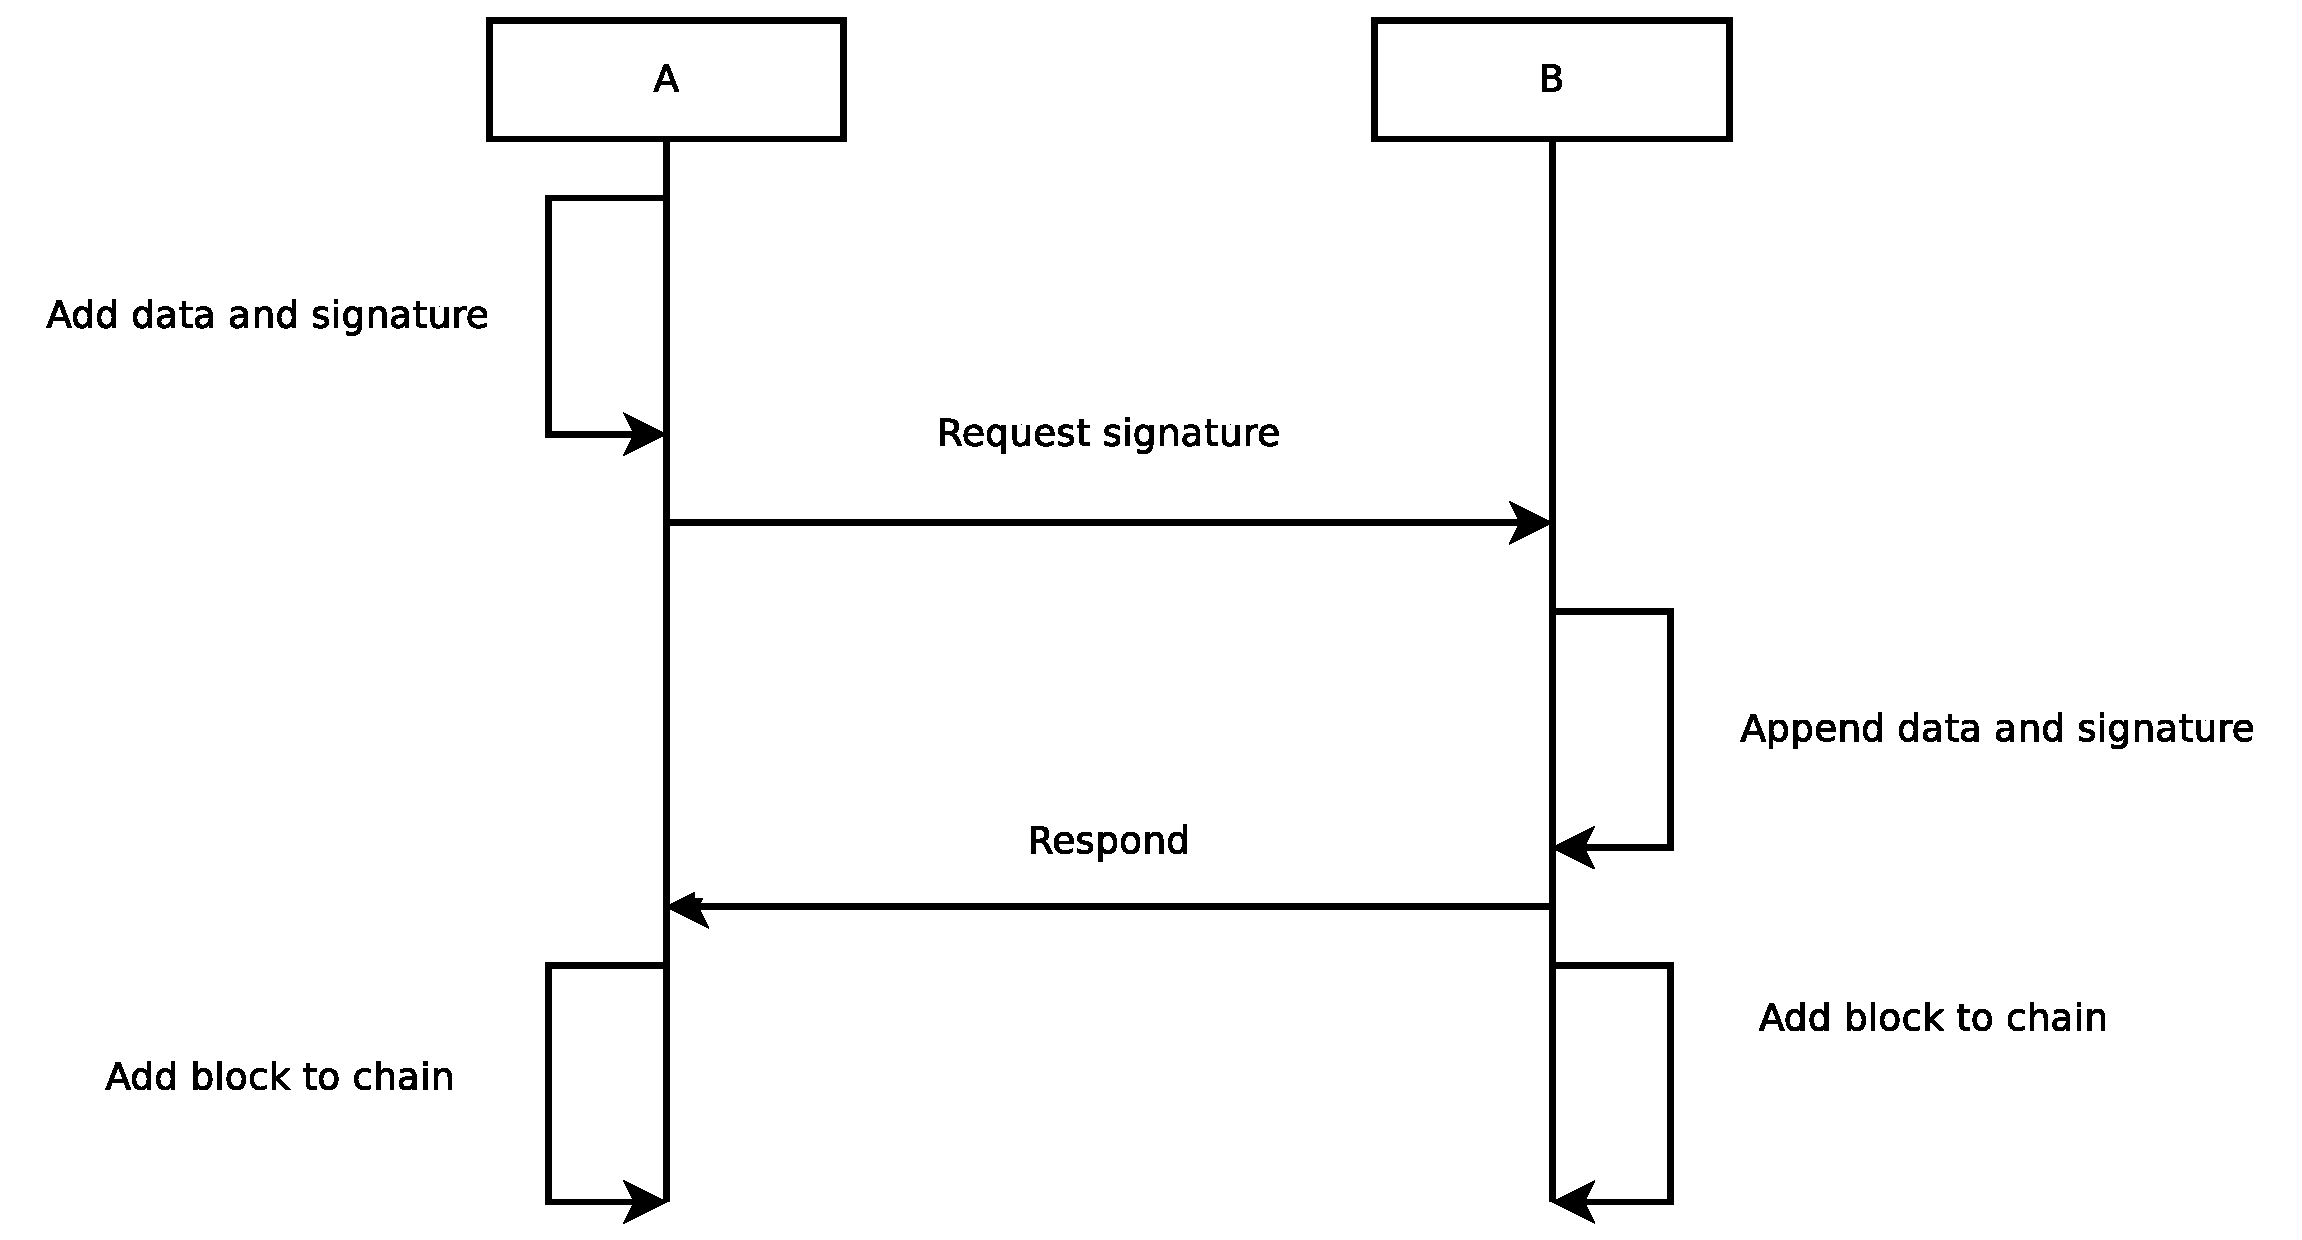
\includegraphics[scale=0.3]{design/figs/exchange_new.eps}}
\label{fig:exchange-new-sequence}
}

\subfigure[Data added by peer A and B for a new block.]{
	\centerline{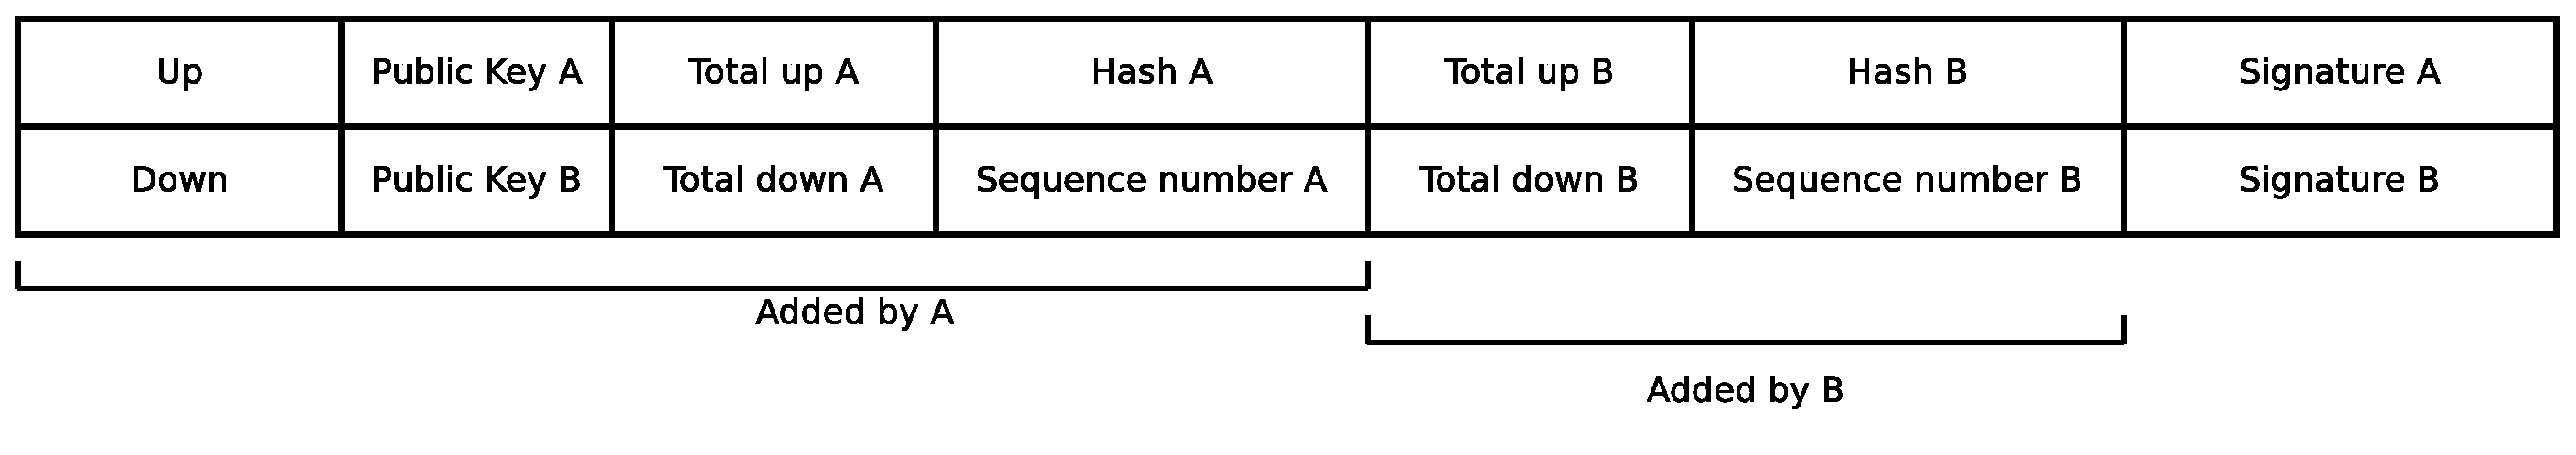
\includegraphics[scale=0.3]{design/figs/packet_creation.eps}}
\label{fig:packet-creation}
}
\caption{Exchanging data for block creation.}
\label{fig:block-creation-new}
\end{figure}

The seeder, A, will create a packet that will be sent to the downloader, B.
A will add to this packet the data uploaded and downloaded data between the peers
that has not yet been added to the MultiChain.
It will add these amounts to its total uploaded and downloaded data
and add these total amounts aswell to the packet.
Finally, it adds the public keys of both peers and its own hash pointer to the packet.
This packet is signed using its private key and sent to the downloader.
The data that A adds can be seen in Figure \ref{fig:packet-creation}.

B will receive this packet and check if the amounts are correct, if the signature is correct,
and if A has not used the previous hash before.
If this is all correct,
then B will add the amounts of uploaded and downloaded data to its own total amounts.
The data contained in the previous packet, the total amounts of B and the hash of the previous block is
inserted into a new packet.
This packet is signed by the private key of B and sent back to A.
The data that B adds can be seen in Figure \ref{fig:packet-creation}.

Both parties now have the data of the block and can add this to their chain and continue forward.
A does this upon receival of the block.
B does this immediatly after sending the return packet to A.
At this point a new block is created.

\subsubsection{Integrating with Dispersy}
\begin{figure}[!h]
\centering
\subfigure[Sequence diagram for block creation.]{
\centerline{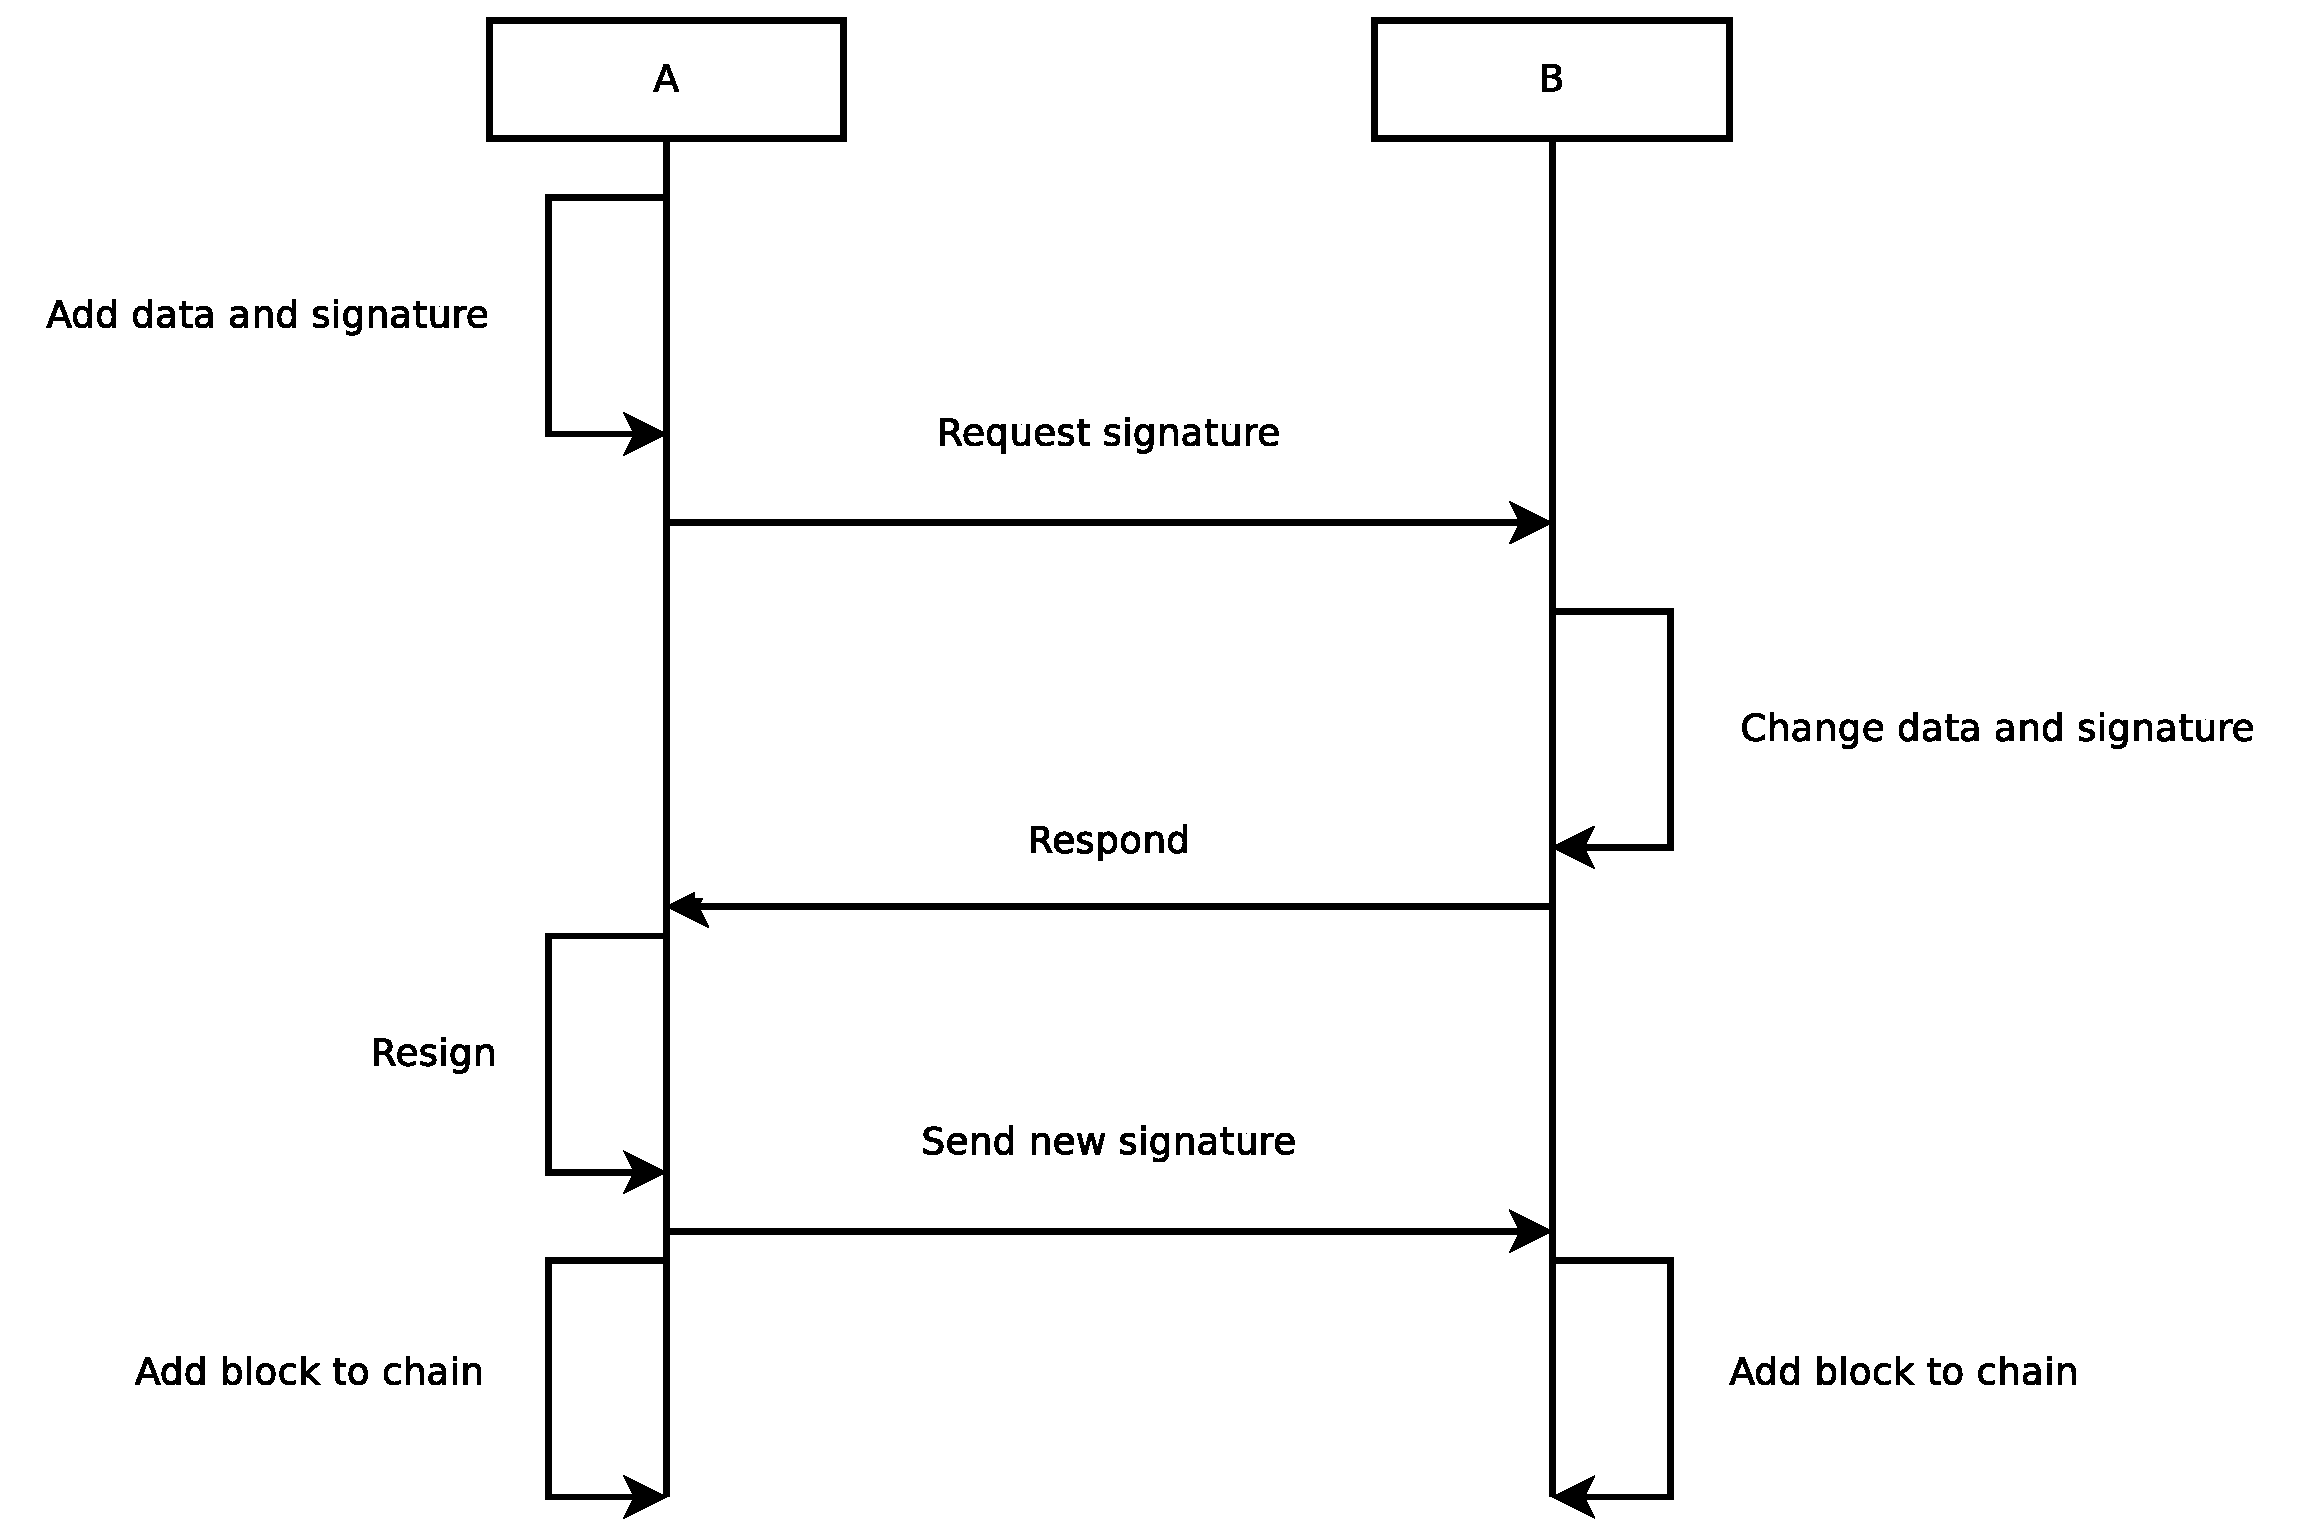
\includegraphics[scale=0.3]{design/figs/exchange_old.eps}}
\label{fig:exchange-old-sequence}
}

\subfigure[Data added by peer A and B for a new block.]{
	\centerline{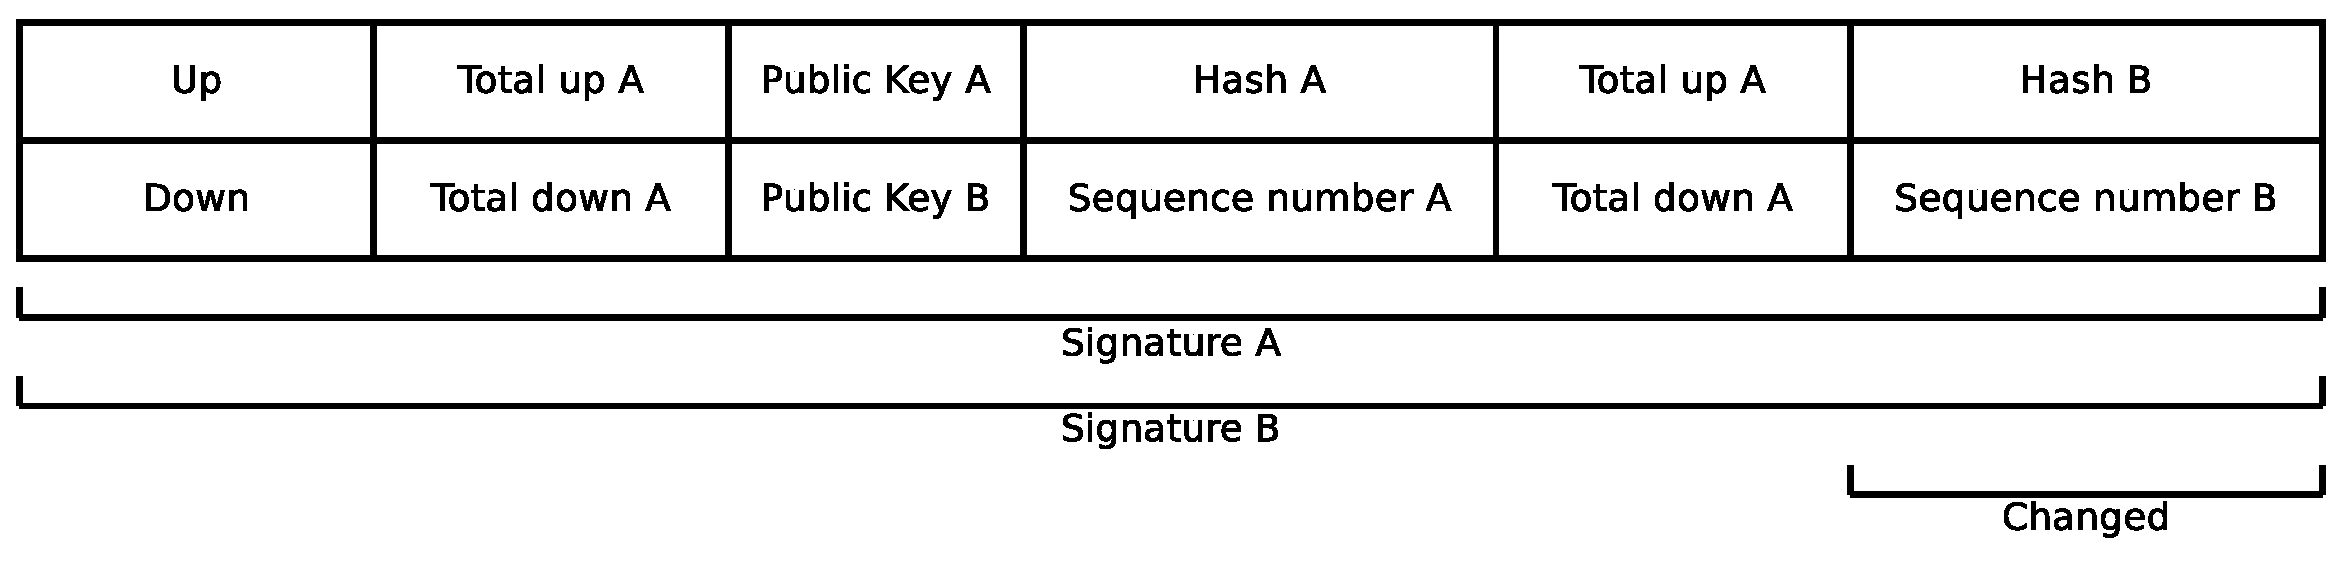
\includegraphics[scale=0.3]{design/figs/signature_old.eps}}
    \label{fig:payload-signature-old}
}
\caption{Exchanging data for block creation using existing functionality.}
\label{fig:block-creation-old}
\end{figure}
Within Dispersy functionality was already build to create a message, sign the message
and request multiple nodes to also provide their signature on this message.
This existing functionality could be used by MultiChain to exchange signatures
between A and B for the creation of a new block.

A would initiate a message, insert its data into this message, sign the message, and send this message to B.
The functionality would allow B to accept the message and provide its signature or
modify the message and then provide its signature.
Only B knows the hash of its head node, and the total up and total download metrics.
So B will always modify the message and insert its own data in the message.
But this would invalidate the signature of A,
because the signature of A was also placed on the empty part of the message where the data of B is inserted.
The contents of the message and who signs what can be seen in Figure \ref{fig:payload-signature-old}.

After B returns the message,
A would have to resign the message.
But B also needs this valid signature from A before it can add the block to its own chain.
So A would need to send a third message to with the new, valid signature back to B.
A sequence diagram can be seen in Figure \ref{fig:exchange-old-sequence} of how it would work in Dispersy.
Functionality was added to Dispersy that allows to append data in a signature request.
This allows the full signature exchange to be achieved within two messages.
\section{Single operations on the chain}
\label{sect:deadlock}
Inside a chain only a single block of a peer is allowed to point to a previous block.
A peer cannot have multiple blocks belonging to him all pointing to the same previous block.
As this is a potential attack as described in section \ref{sect:branch}.
The chain of a peer can only be moved forward by a single block at any time.
Only after a new block is created is the new hash available to be used in the next block.

To ensure this happens correctly the MultiChain community contains mutual exclusive code
that excludes any new operations on the chain if an operation is already pending.
The mutual exclusion is achieved by having to acquire an atomic token to allow to perform an operation on the code.
The MultiChain community will receive incoming signature requests
or requests by other parts of Tribler to send out an outgoing signature request.
The community will decline this request if the token is not available
returns execution to other parts of Tribler.
The token can be unavailable while waiting on another peer in the network to finish responding to a signature request.

\subsection{Circular dependency on the token across peers}
When a MultiChain peer has a pending signature request,
then the peer itself will not respond to incoming signature requests from other peers.
These peers themselves will also not respond as they have a pending signature request.
This can create a circular dependency on the availability of the token.
If two peers send a request to each other at the same time, they will wait on each other.
This could result in a deadlock.

MultiChain prevents this deadlock to occur by allowing a transaction to fail
as explained in section \ref{des:halfsigned}.
If MultiChain gets into this potential deadlock one of the peers will eventually time out of their own signature request
and process the incoming request resolving the circular dependency.
The deadlock is recovered and both peers can continue operation.

This situation has occured during experimentation and it is explained in section \ref{sect:deadlock-exp}.
It is shown that MultiChain correctly recovers the potential deadlock.


\section{Block persistence}
The blocks in the chain have to be persisted to be usable over a prolonged time.
A persistence layer is added to the MultiChain community
that provides all functionality to persist blocks and query blocks.
This layer extends and uses functionality of the Database class in Dispersy.
An overview of the layering in the software architecture can be seen in Figure \ref{fig:persistence-layer}.

\begin{figure}
	\centerline{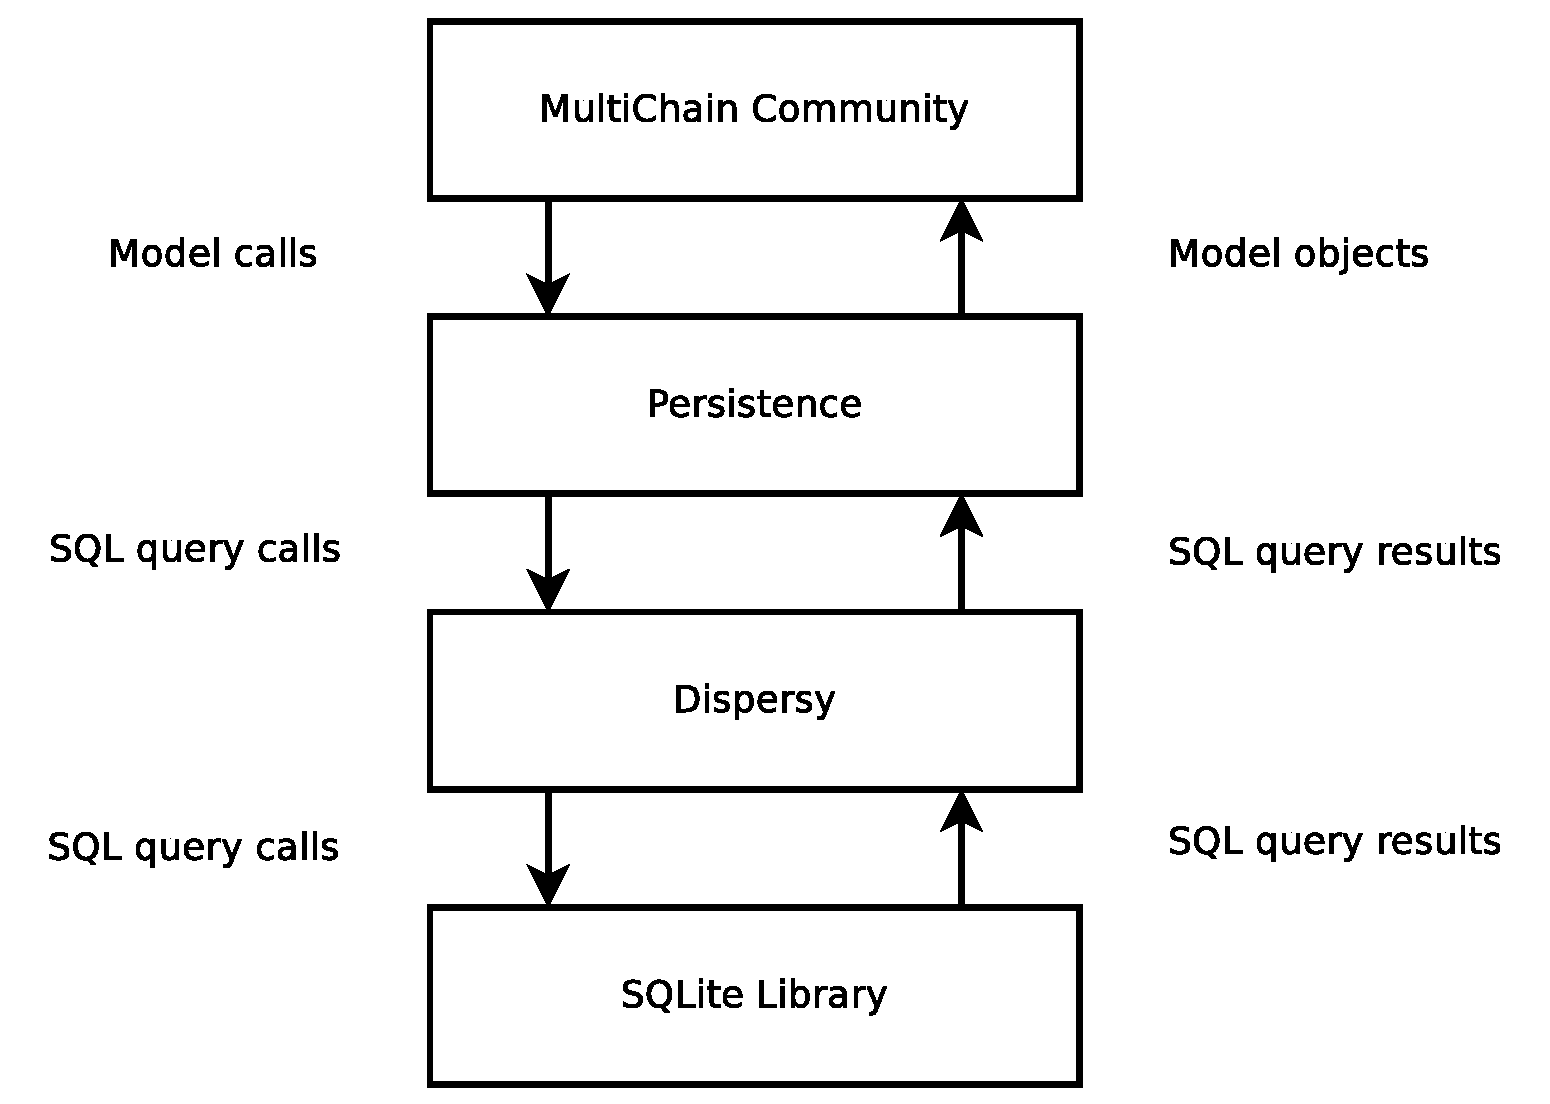
\includegraphics[scale=0.3]{design/figs/persistence-layer.eps}}
	\caption{Persistence layering in the software architecture}
	\label{fig:persistence-layer}
\end{figure}

The MultiChain Community calls functions in the persistence layer that have implicit knowledge about the model.
The Persistence layer formats SQL queries and passes these to the Dispersy layer.
The Dispersy layer performs several sanitation checks and passes these queries to the SQLite Library.
The SQLite Library and Dispersy layer both return the result of the SQL query.
These results are transformed by the Persistence layer into objects of the model usable by the MultiChain Community.

The only information that is saved are blocks.
The information all fits within one table.
A single block is saved as a single record called a row in a relation database.
Every attribute of a block is a single column in the row.
All attributes are saved directly into the database,
except for the public keys.
These public keys are hashed and these hashes are used as an identifier, called mid, in Dispersy.
The public keys are already saved in the Dispersy database.
When a block is retrieved from the database the public key is retrieved from Dispersy using the mid.

Every attribute is queryable in the database.
A public key can be converted to mid and is searched this way.
Every attribute is queryable to make the system  extensible
and usable when the next incremental steps are implemented.
It is presently unknown what information precisly will be needed,
so every information is now made available for the future.

\subsection{Dispersy database}
Dispersy keeps track of information on its own.
A record is kept of any message that can be retrieved using a message id.
The message is saved in a converted format and will be decoded when the message is retrieved.

Instead of storing information in a separate database,
the information could have been retrieved from the Dispersy database.
But the Dispersy database is not queryable.
Because all the information is stored in a converted format
that prevents queries to search the message for its contents.
For this reason, the dispersy database is not used and a separate database is used.

A future, possible improvement to Dispersy would be to save messages queryable in its database.
This would eliminate the current need for separate databases that contain aggregrated information.
The information is stored in two places within Tribler and this could be eliminated.
It would reduce the disk footprint and the amount of read/write transactions
as only one database would have to be maintained.
The I/O ineractions are a problem according to Tribler maintainers.

\section{Crawler}
We implemented a crawler that visits other nodes and request the full chain of that node.
The crawler was built to be used for the experiments and
is a first step in a more sophisticated crawler that will help to solve the known vulnerabilities.
These vulnerabilities will be described in chapter \ref{problems}.

\subsection{Recursively request blocks}
Dispersy provides a list of other nodes that were recently found
and can report when the node itself is found by another node.
Both are sources of destinations nodes that the crawler will visit
and request the chain from.

The crawler will first request from a node the block with sequence number $-1$.
This denotes that he wants the latest block in his chain.
The node returns this block to the crawler.
The crawler will persist the block if it is not yet know.

The newly retrieved block is chained to two blocks with the previous hashes.
The crawler will check if these blocks are present in the database.
If any block is not present,
then the crawler will request that particulair block.
The peer, to whom the block belongs to, has to be known in Dispersy.
If the peer is not known, the block is ignored.
This is done recursively untill the crawler reaches the genesis block of the chain.
In this fashion a breadth first search is implemented for any unknown block
that is present in the chain before the latest block.

The crawl tries to aggregrate as much blocks as possible.
But it gives no certainty that the full MultiChain is collected.
The crawler is able to crawl a disconnected MultiChain,
if for every disconnected partition a peer is known by Dispersy.

\begin{figure}
	\centerline{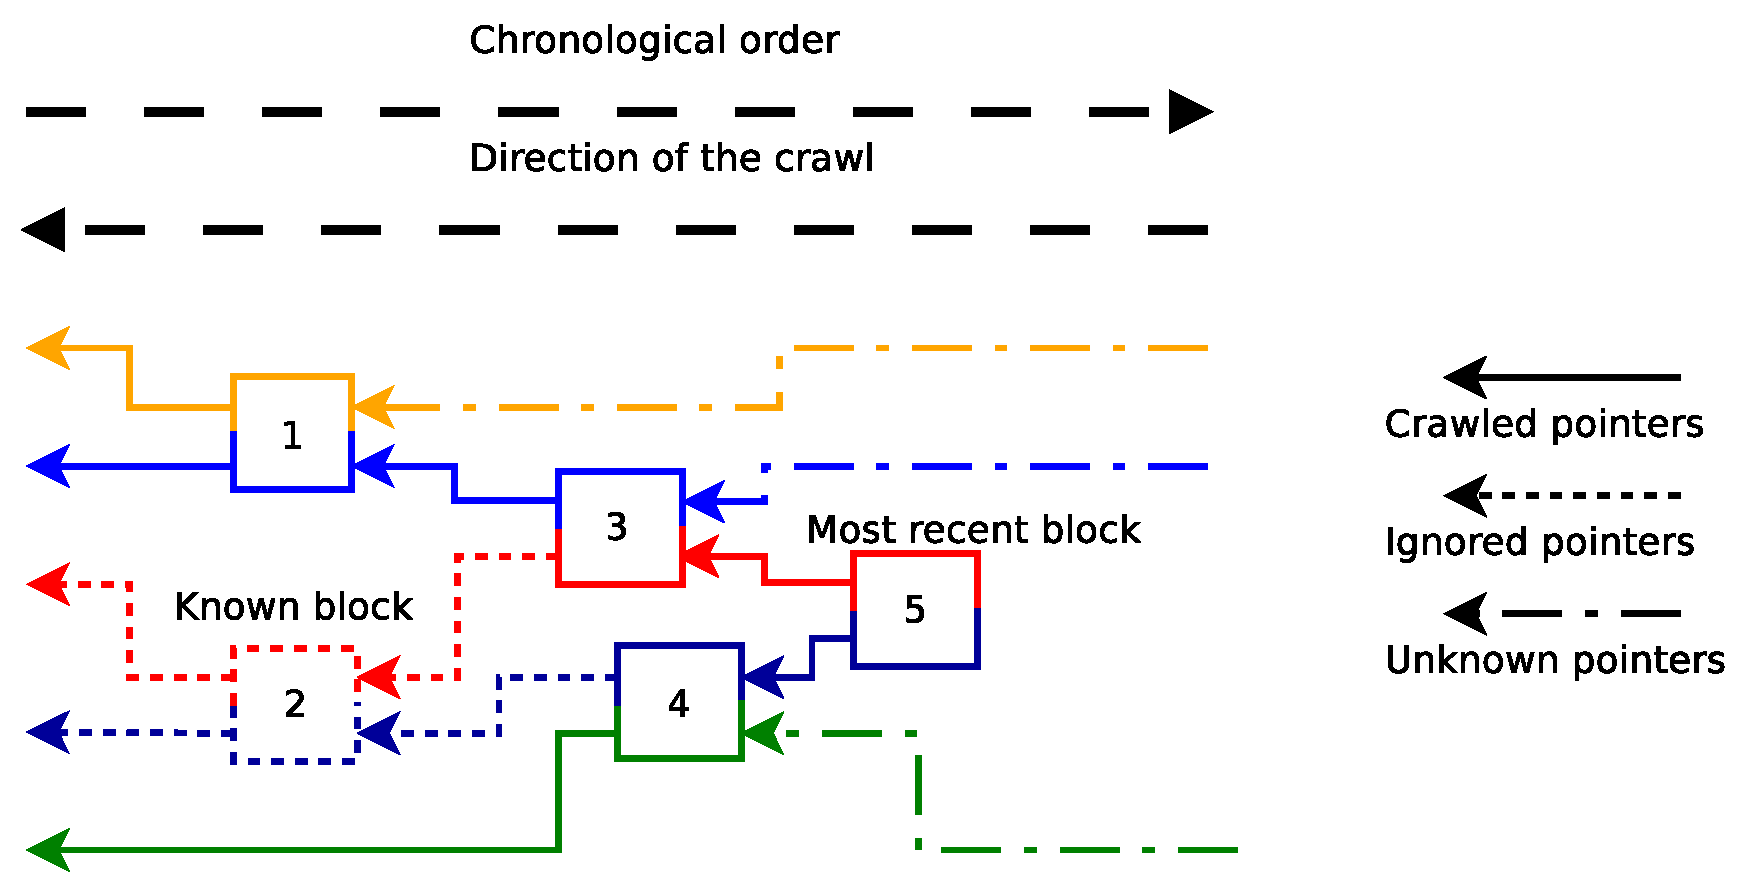
\includegraphics[scale=0.3]{design/figs/crawler-version2.eps}}
	\caption{Example of the crawler looking for unknown blocks. The crawler retrieves the most recent block and crawls older blocks.}
	\label{fig:crawler-example}
\end{figure}

An example can be seen in Figure \ref{fig:crawler-example}.
In this example the line arrows denote paths that the crawler follows,
dotted lines are paths that the crawler ignores,
half dotted lines are paths that the crawler will not know about.
Block 2 is already known by the crawler.
Block 5 is retrieved first by the crawler and the crawler sees hash links to block 3 and 4.
These are retrieved and the block finds links to block 1 and 2.
Because block 2 is already known, it is ignored.
Only block 1 is retrieved.
The crawler continues to follow the links further outside the displayed example.
The half dotted lines are not know by the crawler untill a block is retrieved that contains these paths.
The crawler will retrieve these blocks if for example the most recent block is requested.

\subsection{Recreation over retransmission}
An effort was made to try to reuse code of the community for the crawler and to not introduce another payload type in the community.
The attempt would reuse payload classes and authentication classes already used in the community for the creation of blocks.
This effort failed, because Dispersy cannot handle recreation of messages well
and would invalidate blocks that were recreated.

As said before, Dispersy also keeps tracks of messages received.
The messages containing a block requested by the crawler could be retrieved and retransmissioned forward
instead of being retrieved from the MultiChain database itself.
This would eliminate the need to construct a message and encode the message before it could be send,
because the encoded format is saved and can be retrieved and send immediately.
This was not used as it would be impossible to distinguish messages received as an response to a signature request or a crawler request.
The two types of responses cannot be processed in the same way.
A response to a signature requests has to influence the way a node responds to interactions
and a crawler response should not.

In the end, the crawler uses recreation of a block from the local database and uses a new payload type to forward blocks.
The main reasons this implementation was chosen is
that implemenation was very simple and had none of the above mentioned problems.
Maintainabillity is also much easier this way
as different types of messages are not using the same functions to be received in the code.
This might not be known by a new programmer working with the code.

\subsection{Improvements}
The crawler is a first, simple step towards a more sophisticated crawler.
Tribler has implemented already more sophisticated crawlers for Bartercast
and these techniques can be reused for the MultiChain crawler.
For example bloom filters can be used in conjunction with the knowledge
that every record is a part of the chain to quickly request multiple blocks\cite{broder-bloomfilter}\cite{logiotatidis-splash}.
Blocks could also be send in a more efficient way by sending multiple blocks per message.
Secondly, blocks that belong to a different node than the crawled node are requested,
but the location of this different node is only known by chance.
Dispersy only keeps track of 20 peers at any time, so the chance is low that the node is among these nodes.
The chance can be improved by asking if the first contacted node knows the location of the different node.




%Experimentation
\chapter{Implementation and experiments}
The design of MultiChain in the previous chapter has been fully implemented.
In this chapter we test if MultiChain is correctly implemented according to the design
and we experiment the MultiChain in various scenarios.
MultiChain is experimented with to test if it can correctly create a chain tracking a download.
Next, MultiChain is experimented with tracking anonymous downloads.
Finally, MultiChain is experimented with in potential situations where a deadlock may occur
to test if it succesfully resolve these situations.

In this chapter multiple graphs are depicted.
These graphs are generated by reading every database of every node.
The blocks are depicted as nodes and the previous hash pointers are edges in the graph.
The nodes have added colouring to indicate extra meaning.
This can be seen in Figure \ref{fig:graph-example}
Green nodes are a first block in a MultiChain of a peer,
and as such have no inbound arrows.
Blue nodes are a sequential block between the same previous peers,
therefore they do not have two inbound arrows.
Red nodes are half-signed blocks,
and therefore only have one inbound and one outbound arrow.

\begin{figure}[!h]
	\centerline{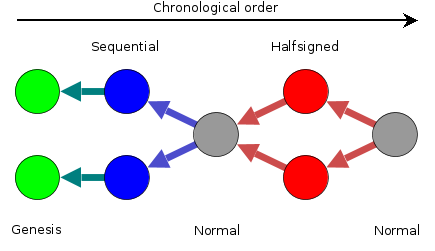
\includegraphics[scale=0.6]{experimentation/example.png}}
	\caption{Example of coloring used in Figures with graphs.}
	\label{fig:graph-example}
\end{figure}

Some experiments were also run multiple times because Dispersy does not always connect to every peer.
At the start of the experiment the peers are forced to be introduced,
but this does not always succeed.
This is a problem in discoverability and has been experienced by previous work aswell~\cite{ruigrok-anonymous}.
The final version is chosen when Dispersy did connect all the peers.
We recommend that Dispersy is changed to allow a modified behaviour when experimenting
where the pool of candidates is not refreshed,
as explained in section \ref{sect:bartercast}

\section{Software engineering tests}
MultiChain is tested in several ways to verify it is correctly working
following standard software engineering practices.
The enforcement of these types of tests is a policy recently introduced within Tribler.

\subsection{Unit Tests \& Integration tests}
Tribler uses Python unit tests to validate small components of code.
The tests can be run locally and
are automatically run on a Jenkins build server\cite{jenkins}\cite{jenkins-tribler}.
Unit tests were added to increase stability of MultiChain.
Integration tests were added to test multiple components of MultiChains working integrated together.

Tribler does prove to be hard to test using unit tests.
This is due to high coupling of code within Tribler.
But mocking of classes helped in testing difficult to test code.
The separate unit tests for the conversion, payload and database were the first of it types inside Tribler.
Also Dispersy was expanded to introduce new functionality to make it easier to create unit tests for communities in the future.
An overview of the coverage can be seen in Table \ref{tab:tests}
In the end a high level of testing has been achieved, especially in comparison to the rest of Tribler.
The total test coverage of Tribler was only 16\% at time of writing\cite{jenkins-tribler}.
A decision using code coverage tools was made that the untested code has little value to further test in comparison to the work required.
The code was tested in Gumby scenarios.

\begin{table}
\centering
\begin{tabular}{l|ll|ll}
Filename   & LOC & \% covered   & Conditionals & \% covered    \\ \hline
Community  & 187 & 81\%         & 37           & 95\%  \\
Conversion & 60  & 100\%        & 6            & 100\%  \\
Database   & 100 & 100\%        & 6            & 84\%  \\
Payload    & 89  & 100\%        & 2            & 100\% \\ \hline
Total      & 672 &              & 47           &
\end{tabular}
\caption{Unit tests coverage of MultiChain.}
\label{tab:tests}
\end{table}

\subsection{Gumby}

Next to that, Tribler uses a homemade test runner Gumby.
Gumby can start multiple instances of Tribler and follow test scenarios.
Gumby can be used to perform system tests and experiments.
These system tests have to be manually validated.
Several scenarios have been written to validate MultiChain.
These run MultiChain either in a standalone version or integrated into the TunnelCommunity.

One of these scenarios can be found in Figure \ref{fig:exp-gumby-scenario}
In this example basic block creation is tested.
Normal situations are tested,
but also situations where the signature requests are answered late
and other requests arrive at the requesting peer at the same time.
Additionally, signature requests are controlled to not be answered at all.
During the whole test the crawler is active and scrapes the network for unknown blocks.
The notation in the scenario is the time an action has to be taken place,
the action that has to be taken, and by who if necessary.
The "@0:" can be ignored, but is required in the Gumby format.

\begin{figure}
\begin{FVerbatim}[fontsize=\small]
@0:0 set_master_member 3081a7301006072a8648ce ... 2b51
@0:0 set_community_class MultiChainNoResponseCommunity {4}
@0:0 set_community_class MultiChainDelayCommunity {5}
@0:0 set_community_class MultiChainCommunityCrawler {6}
@0:0 set_community_class {6}
@0:0 start_dispersy
@0:1 online
@0:5 reset_dispersy_statistics
@0:10 annotate start-experiment-1-peer
@0:15 introduce_candidates
@0:80 request_signature 2 {1}
@0:84 request_signature 1 {2}
@0:94 request_signature 4 {1}
@0:95 request_signature 1 {3}
@0:104 request_signature 5 {1}
@0:106 request_block 1 5 {6}
@0:110 close
@0:111 stop_dispersy
@0:112 stop
\end{FVerbatim}
    \caption{One of the Gumby definition files.}
    \label{fig:exp-gumby-scenario}
\end{figure}

\section{Tracking download and upload amounts}
In this section we will experiment with MultiChain creating blocks and tracking download and upload amounts of peers.
We will first start with creating a simple block in an experiment.
The next experiment is to try to create a chain of blocks with mimicking a download of 10MB
and a larger download of 10GB.
Downloads are done at different download speeds and an experiment was done to test MultiChain in this environment.

\section{Single block creation}
In this experiment we try to create a block between two nodes.
This experiment validates the MultiChain to be able to correctly create a block between nodes in normal circumstances.
The experiment is locally run using gumby with all nodes running on a single computer.
Only two instances of MultiChain communities are started and between these two communities a block is created.
The logging of the both nodes is captured and recorded to verify the results of the experiment.

The output of the logging can be seen in figure \ref{fig:singleblockexperiment}.
First node 1 sends a signature request to node 2.
This message is received and a block is persisted.
The hash of the block is displayed in the output.
The block is sent back as a signature response to node 1.
The block is saved by node 1 and has the same hash as shown in the output.
So the block between node 1 and node 2 is the same and a block was succesfully created.
The output also shows behaviour of MultiChain
to correctly exclude any other execution from entering mutual exclusive code.
The lines related to the mutual exclusion are prepended by "Chain Excl".
The nodes check if it is possible to enter the mutual exclusive part and correctly acquires
and releases the mutual exclusion token.

\begin{figure}
\begin{FVerbatim}[fontsize=\small]
1: Requesting Signature for candidate: 2
1: Chain Exclusion: signature request: False
1: Chain Exclusion: acquired, sending signature request.
1: Sending signature request.
2: Received signature request.
2: Chain Exclusion: process request: False
2: Chain Exclusion: acquired to process request.
2: Persisting sr: 2F7bTMxyJU7hZkvaBimT2bYm4bY=
2: Chain Exclusion: released after processing request.
2: Sending signature response.
1: Signature response received. Modified: True
1: Valid 1 signature response(s) received.
1: Persisting sr: 2F7bTMxyJU7hZkvaBimT2bYm4bY=
1: Chain exclusion: released received signature response.
\end{FVerbatim}
    \caption{Output of single block creation experiment}~\label{fig:singleblockexperiment}
\end{figure}

\subsection{Chaining blocks}
The next experiment we experiment with MultiChain creating a chain of blocks between two peers.
The experiment is run using gumby with all peers running on a single computer.
We try to create 10 subsequent blocks mimicking a download of 10MB with a speed of 1000 KB/s.
Every second these amounts are indicated to have been transferred to the schedulers of every peer.
The scheduler waits for 1MB uploaded to another peer before scheduling a block.

The result of the experiment can be seen in the graph in Figure \ref{fig:chain-experiment-graph}.
In this graph it can be clearly seen that MultiChain is succesful in creating a chain of 10 blocks.

\begin{figure}[!h]
	\centerline{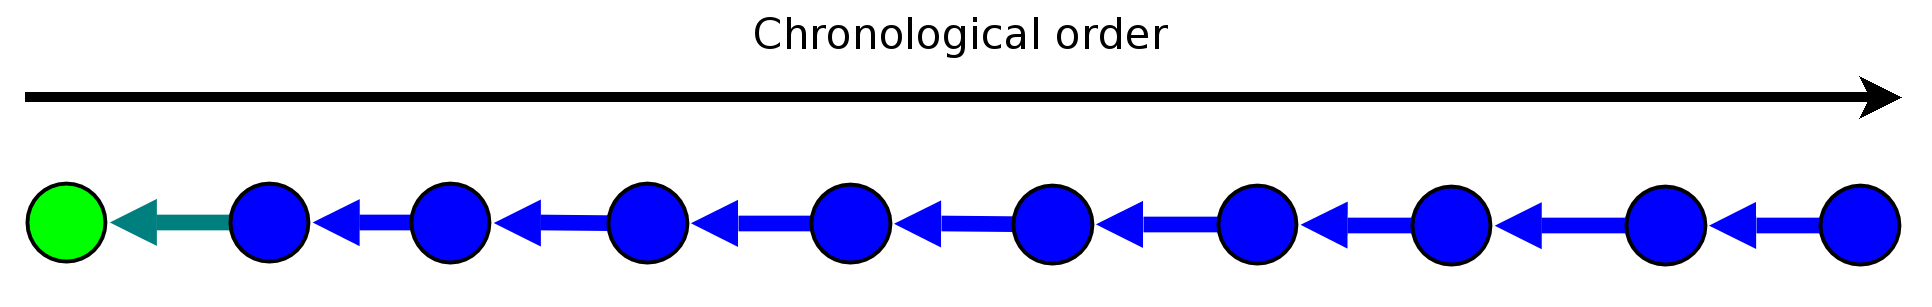
\includegraphics[scale=0.6]{experimentation/chain/chain.png}}
	\caption{MultiChain chain graph of a single download of 10 MB.}
	\label{fig:chain-experiment-graph}
\end{figure}

The amounts stored in each blocks are plotted in Figure \ref{fig:chain-experiment-amounts}.
Every datapoint is a block in the chain of a peer and is the the total amount stored in that block..
These datapoints are connected by a dotted line representing the link between these blocks.
These plots show that MultiChain correctly tracks the download of 10MB.
The slope of the figure corresponds with the speed of the download.

\begin{figure}
\centering
\subfigure[Total download amount.]{
\centerline{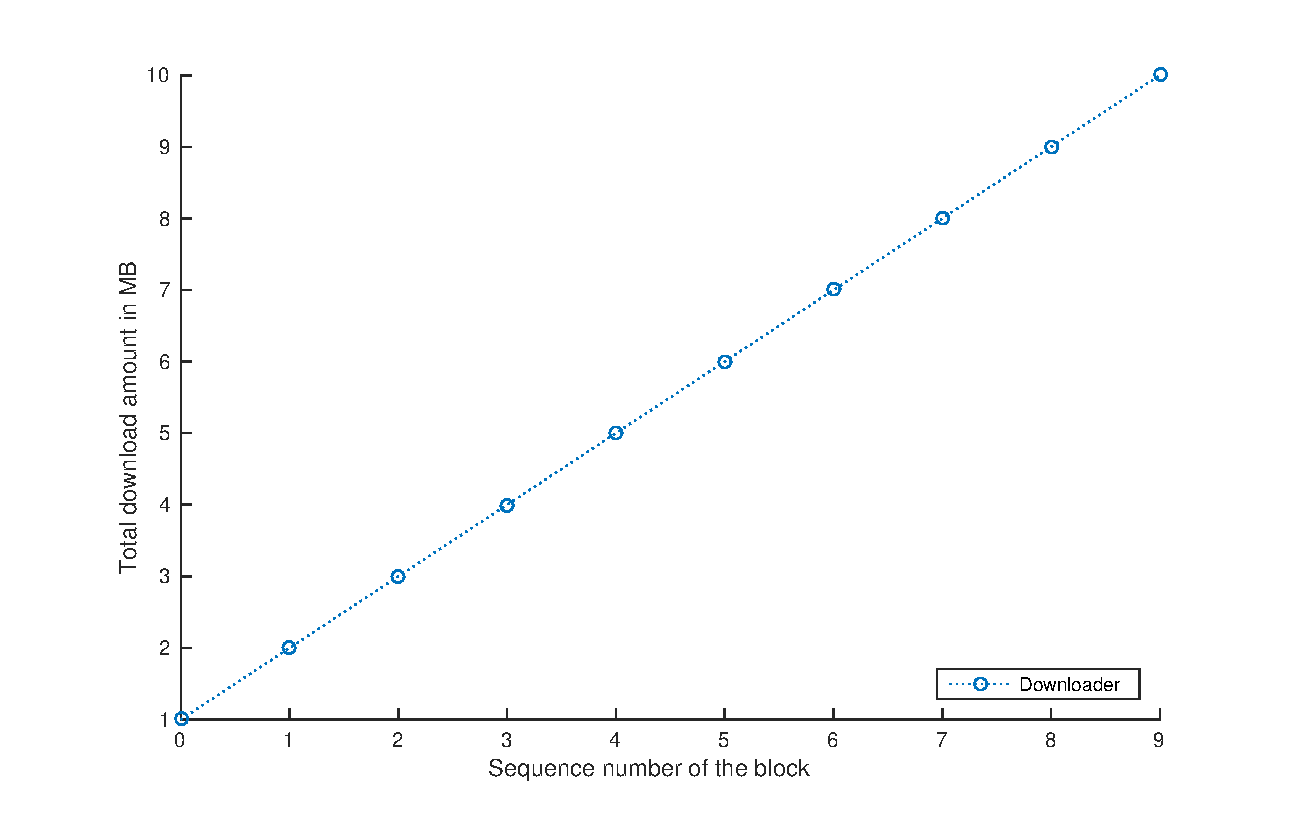
\includegraphics[scale=0.5]{experimentation/chain/chain-down.eps}}
\label{fig:chain-experiment-down}
}
\subfigure[Total upload amount.]{
\centerline{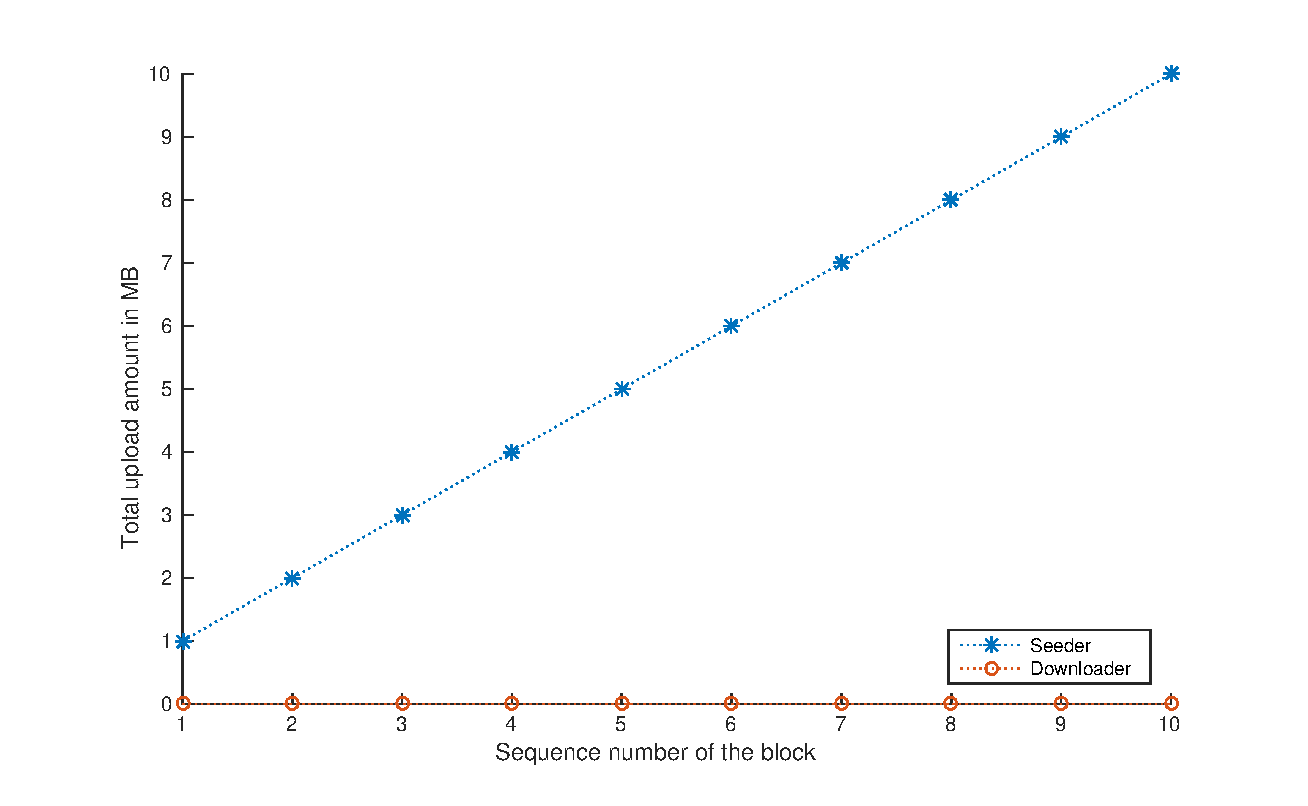
\includegraphics[scale=0.5]{experimentation/chain/chain-up.eps}}
\label{fig:chain-experiment-up}
}
\caption{Download and upload amounts when creating a chain of 10 blocks.}
\label{fig:chain-experiment-amounts}
\end{figure}

\subsection{Tracking downloads with different speeds}
In this experiment we measure if MultiChain can correctly track the upload and download amounts
between two peers with different speeds.
In the scenario a file of 100 MB is downloaded at different speeds,
respectively 500 KB/s, 750 KB/s, 1000 KB/s, 1250 KB/s, 2000 KB/s, and 3000 KB/s.
The maximum speed of anonymous download was measured in experiments to be 1150 KB/s\cite{ruigrok-anonymous}.
The scheduler waits for 1MB uploaded to another peer before scheduling a block.
The upload and download of the file is done by different pairs of seeders and leechers.
Every second these amounts are indicated to have been transferred to the schedulers of every peer.

\begin{figure}
\centering
\subfigure[Total download amount.]{
\centerline{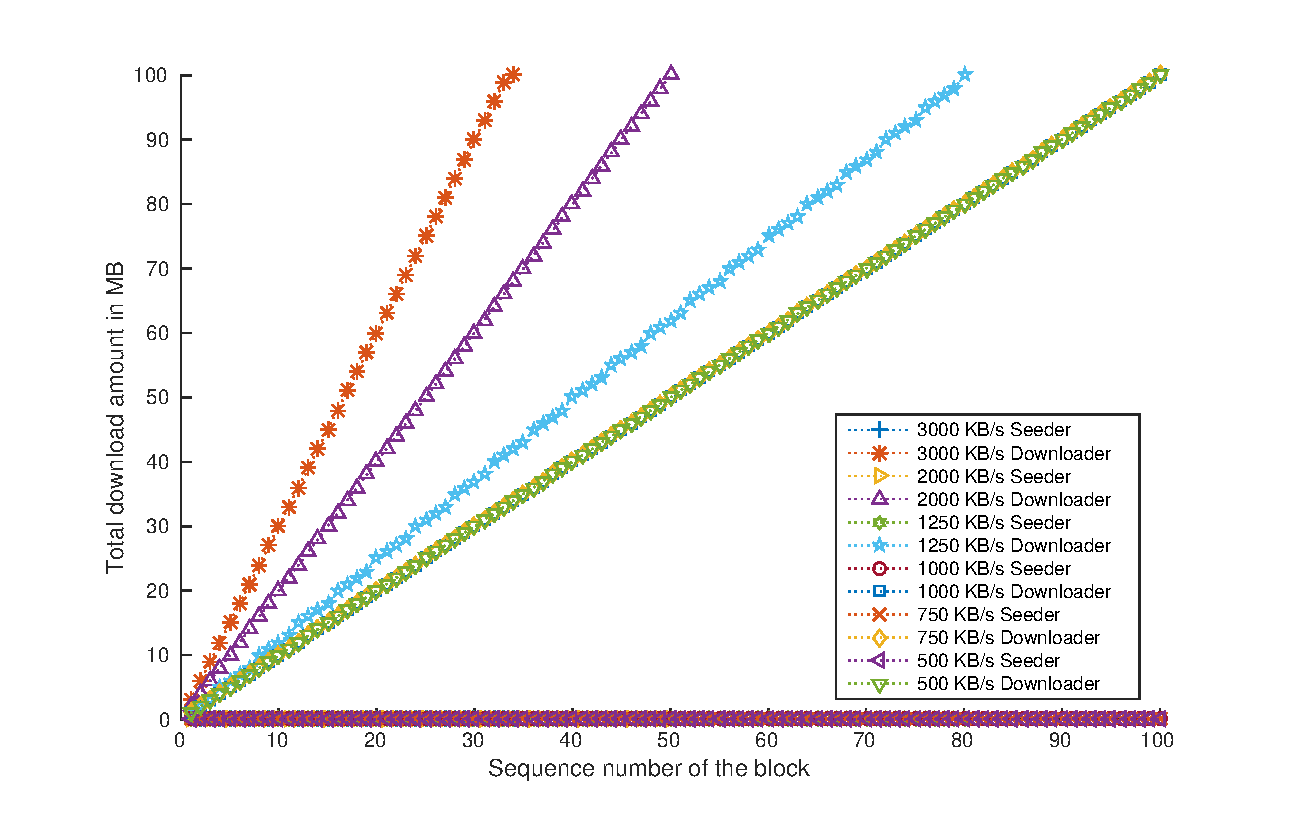
\includegraphics[scale=0.5]{experimentation/speeds/synthetic-simple-down.eps}}
\label{fig:synthetic-simple-down}
}
\subfigure[Total upload amount.]{
\centerline{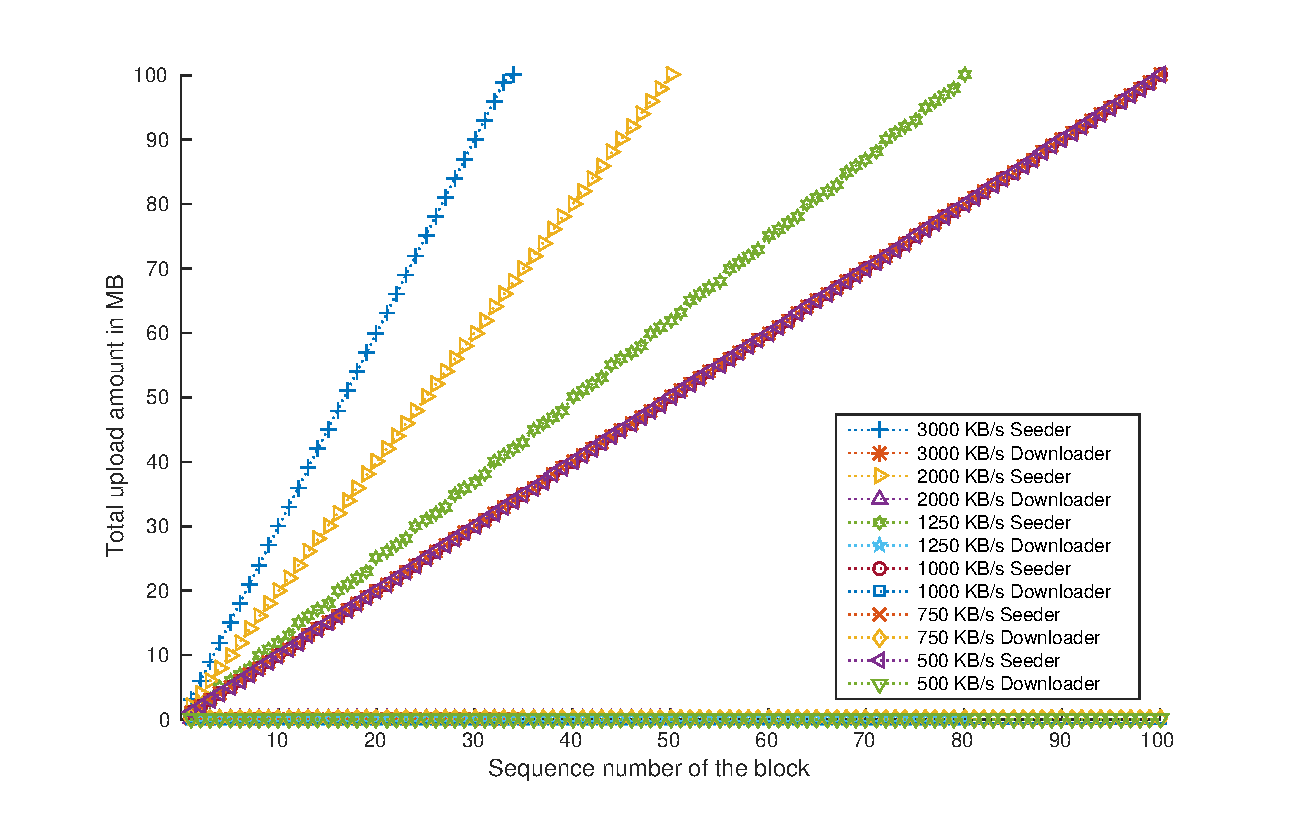
\includegraphics[scale=0.5]{experimentation/speeds/synthetic-simple-up.eps}}
\label{fig:synthetic-simple-up}
}
\caption{Download and upload amounts when tracking downloads at different speeds.}
\label{fig:synthetic-simple-amounts}
\end{figure}

The total download and upload amounts of every peer is plotted in Figure \ref{fig:synthetic-simple-amounts}.
These amounts are plotted in the same way as the previous experiment.
The plots show that MultiChain is able to correctly track the download and upload amounts without a problem.
There are no hitches in the figures and the amounts go up in fixed increments corresponding to the different speeds.
This means that MultiChain is fast enough to correctly track the amounts.

The download speeds below the threshold of 1000 MB of the scheduler
are not distinguishable from the download at the threshold speed.
This is because the scheduler waits until the threshold is reached before initiating the block.
The amount is tracked in the same amount of blocks,
but the total time of the experiment is longer for these experiments.
If the speed goes above the threshold, then this is reflected in the figure.

The graph in Figure \ref{fig:synthetic-simple-graph} shows the graph of the blocks created by the experiment.
The graph is disconnected, because the different pairs of seeders and leechers did not interact with each other.
So no block that would connect their chains is created,
This leaves the graph disconnected.

\begin{figure}
	\centerline{
\includegraphics[scale=0.06]{experimentation/speeds/synthetic.png}}
	\caption{Disconnected chain graph of 6 individual downloads at different speeds.}
	\label{fig:synthetic-simple-graph}
\end{figure}

This experiment was run several times before the final version in this report was run.
Earlier versions of the experiment resulted in two bugfix and two improvements:
the ability of the scheduler to create a block at the end of a download.

\section{Tracking anonymous data transfer}
In this section we will experiment with MultiChain tracking anonymous data transfer.
Anonymous data transfer is a more complicated environment,
where multiple peers work together to transfer data from the seeder to the leecher.
We experiment in a synthetic environment and in environment using real anonymous downloads between peers.

\subsection{Anonymous download}
In an anonymous download scenario the data is downloaded through multiple hops.
A seeder uploads data to the first hop.
This hop passes the data to the second hop.
The second hop sends the data to its destination at the leecher.
This can be seen as sequence of peers and is illustrated in Figure \ref{fig:seeder-hops-leecher}.
More hops can be added to better safegaurd the anonymity of the download.

\begin{figure}
	\centerline{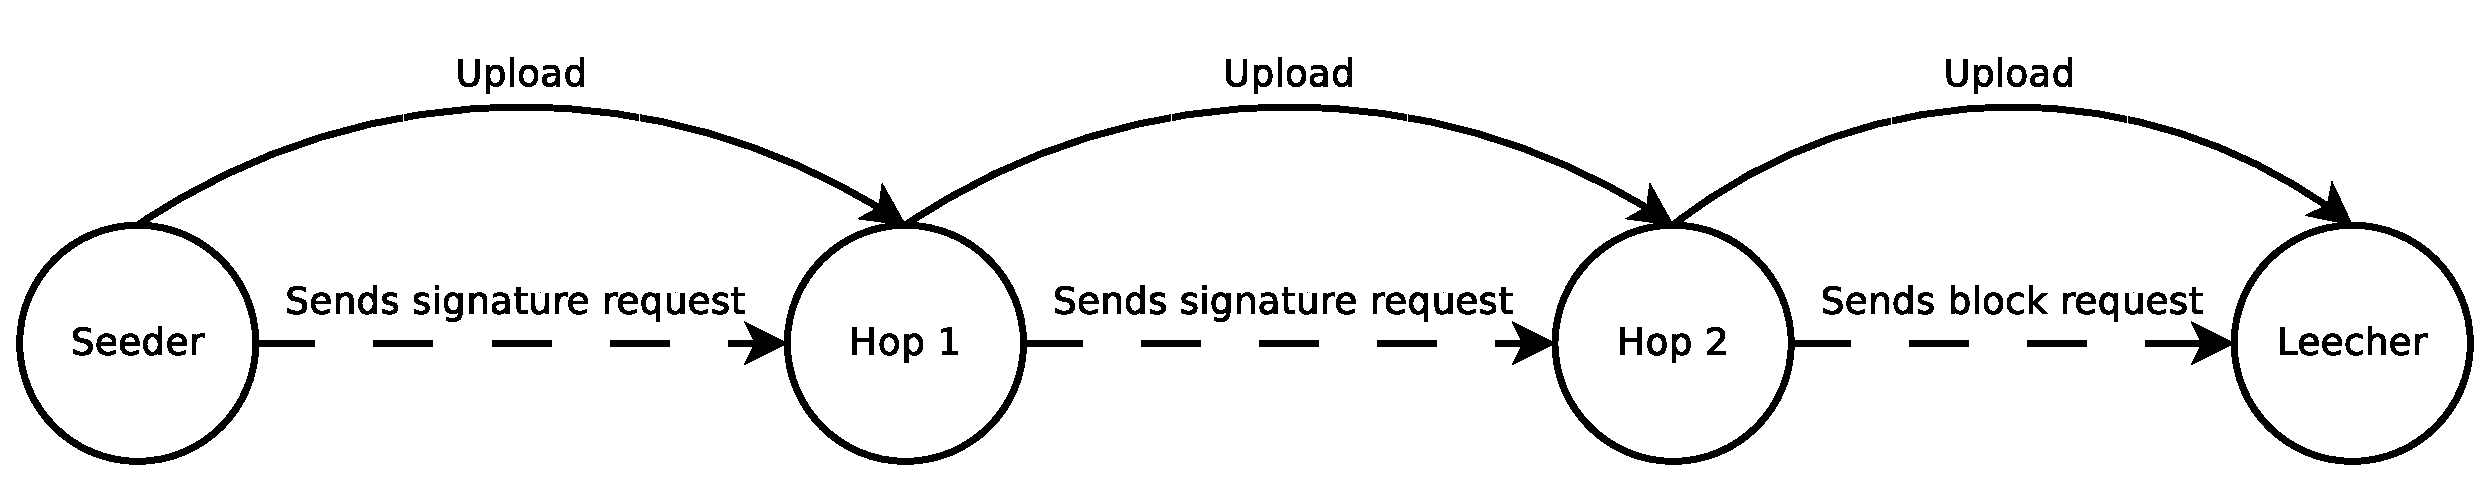
\includegraphics[scale=0.3]{experimentation/anonymous/seeder-hops-leecher.eps}}
	\caption{Block creation in an anonymous download.}
	\label{fig:seeder-hops-leecher}
\end{figure}

The total download and upload amount is plotted, in the same way as the previous experiment,
in Figure \ref{fig:synthetic-anonymous-amounts}.
The slopes of the figures are not representative for the upload and download speeds of the peers.
This is because the x-axis represents the sequence-number of the block and not time.
The hops create blocks that can be categorized in two types:
a download validating block and an upload validating block.
The download validating block only contains information about how much the hop has downloaded
and is initiated by the peer in front of the peer in the sequence.
An upload validating block is initiated by the peer itself with the peer next in the sequence.
The seeder only has upload validating blocks and as such has half the amount of blocks.
The downloader has viceversa only download validating blocks.
The slope of his figure is much steeper as a result.

In the graph a hitch can be found in the figures of the seeder and the first hop.
This is the result of the first hop sending a signature request to the second hop.
The second hop was not able to process this request,
because it was already working on creating another block.
The first hop will still wait on the second hop to process its request untill it will timeout.
In turn, the seeder sent a request to the first hop that will timeout,
because the first hop is not able to process this request aswell.
During the timeouts of the seeder and the first hop,
the second hop continues to validates its own upload amounts.
No blocks are created that validate his download amount,
so the slope becomes steeper during that time and the download amount remains level.
The timeouted peers create no blocks.
When the timeouts expires, the system returns to function as normal.
In section \ref{sect:deadlock-exp} we further experiment with the timeouts in the system.

\begin{figure}
\centering
\subfigure[Total download amount.]{
\centerline{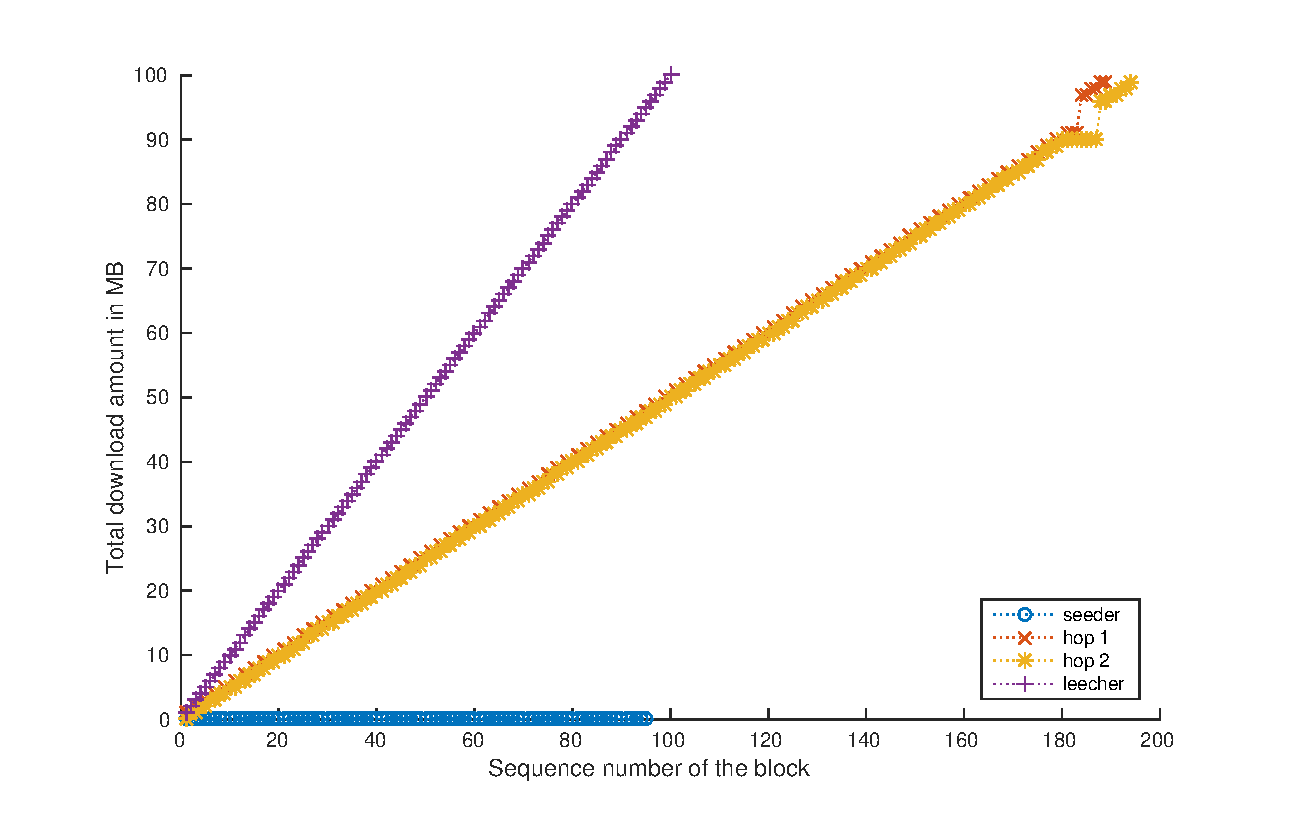
\includegraphics[scale=0.5]{experimentation/anonymous/synthetic-anonymous-down.eps}}
\label{fig:synthetic-anonymous-down}
}
\subfigure[Total upload amount.]{
\centerline{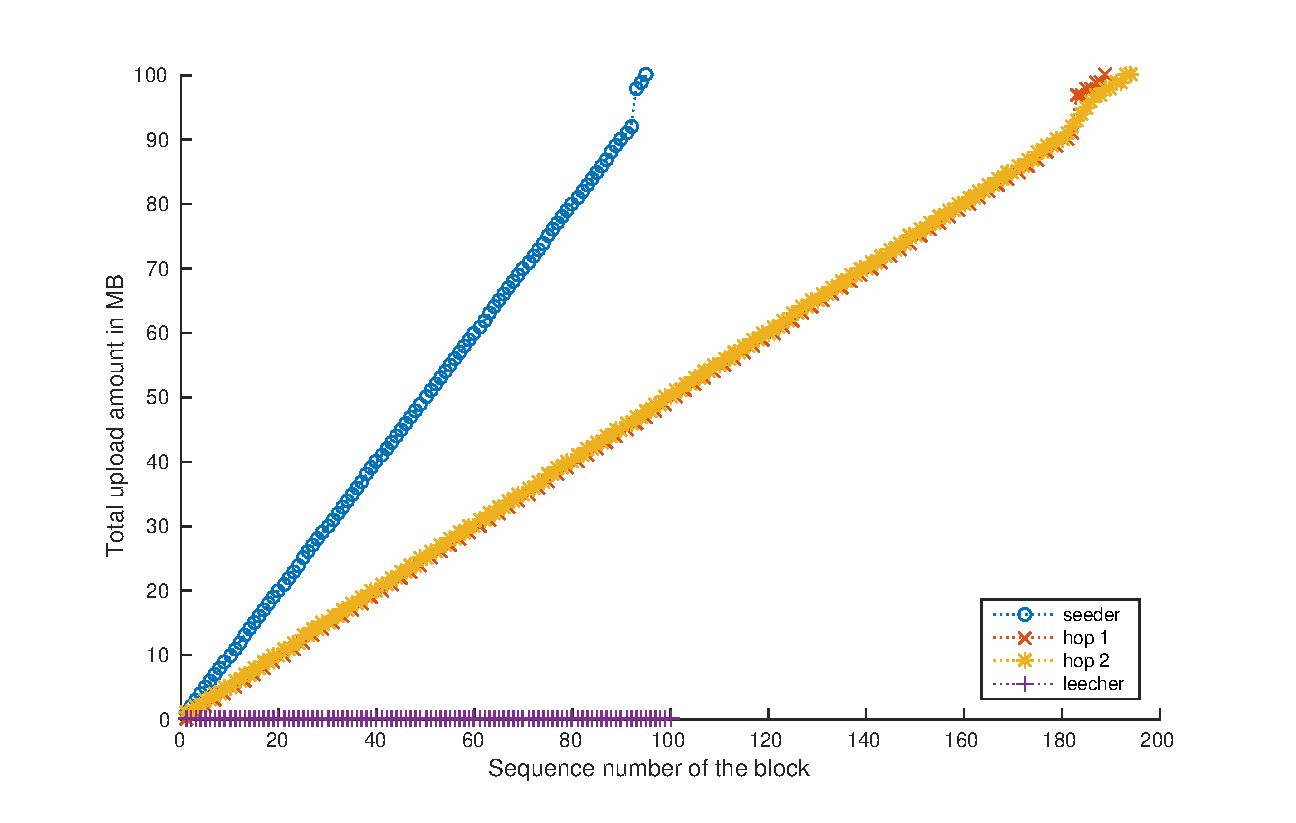
\includegraphics[scale=0.5]{experimentation/anonymous/synthetic-anonymous-up.eps}}
\label{fig:synthetic-anonymous-up}
}
\caption{Download and upload amounts during the anonymous download experiment.}
\label{fig:synthetic-anonymous-amounts}
\end{figure}

The graph in Figure \ref{fig:synthetic-anonymous-graph} shows the graph of the blocks created by the experiment.
In contrast to the previous experiment, this graph is connected.
Because every peer interacts indirectly with every other peer.

\begin{figure}
	\centerline{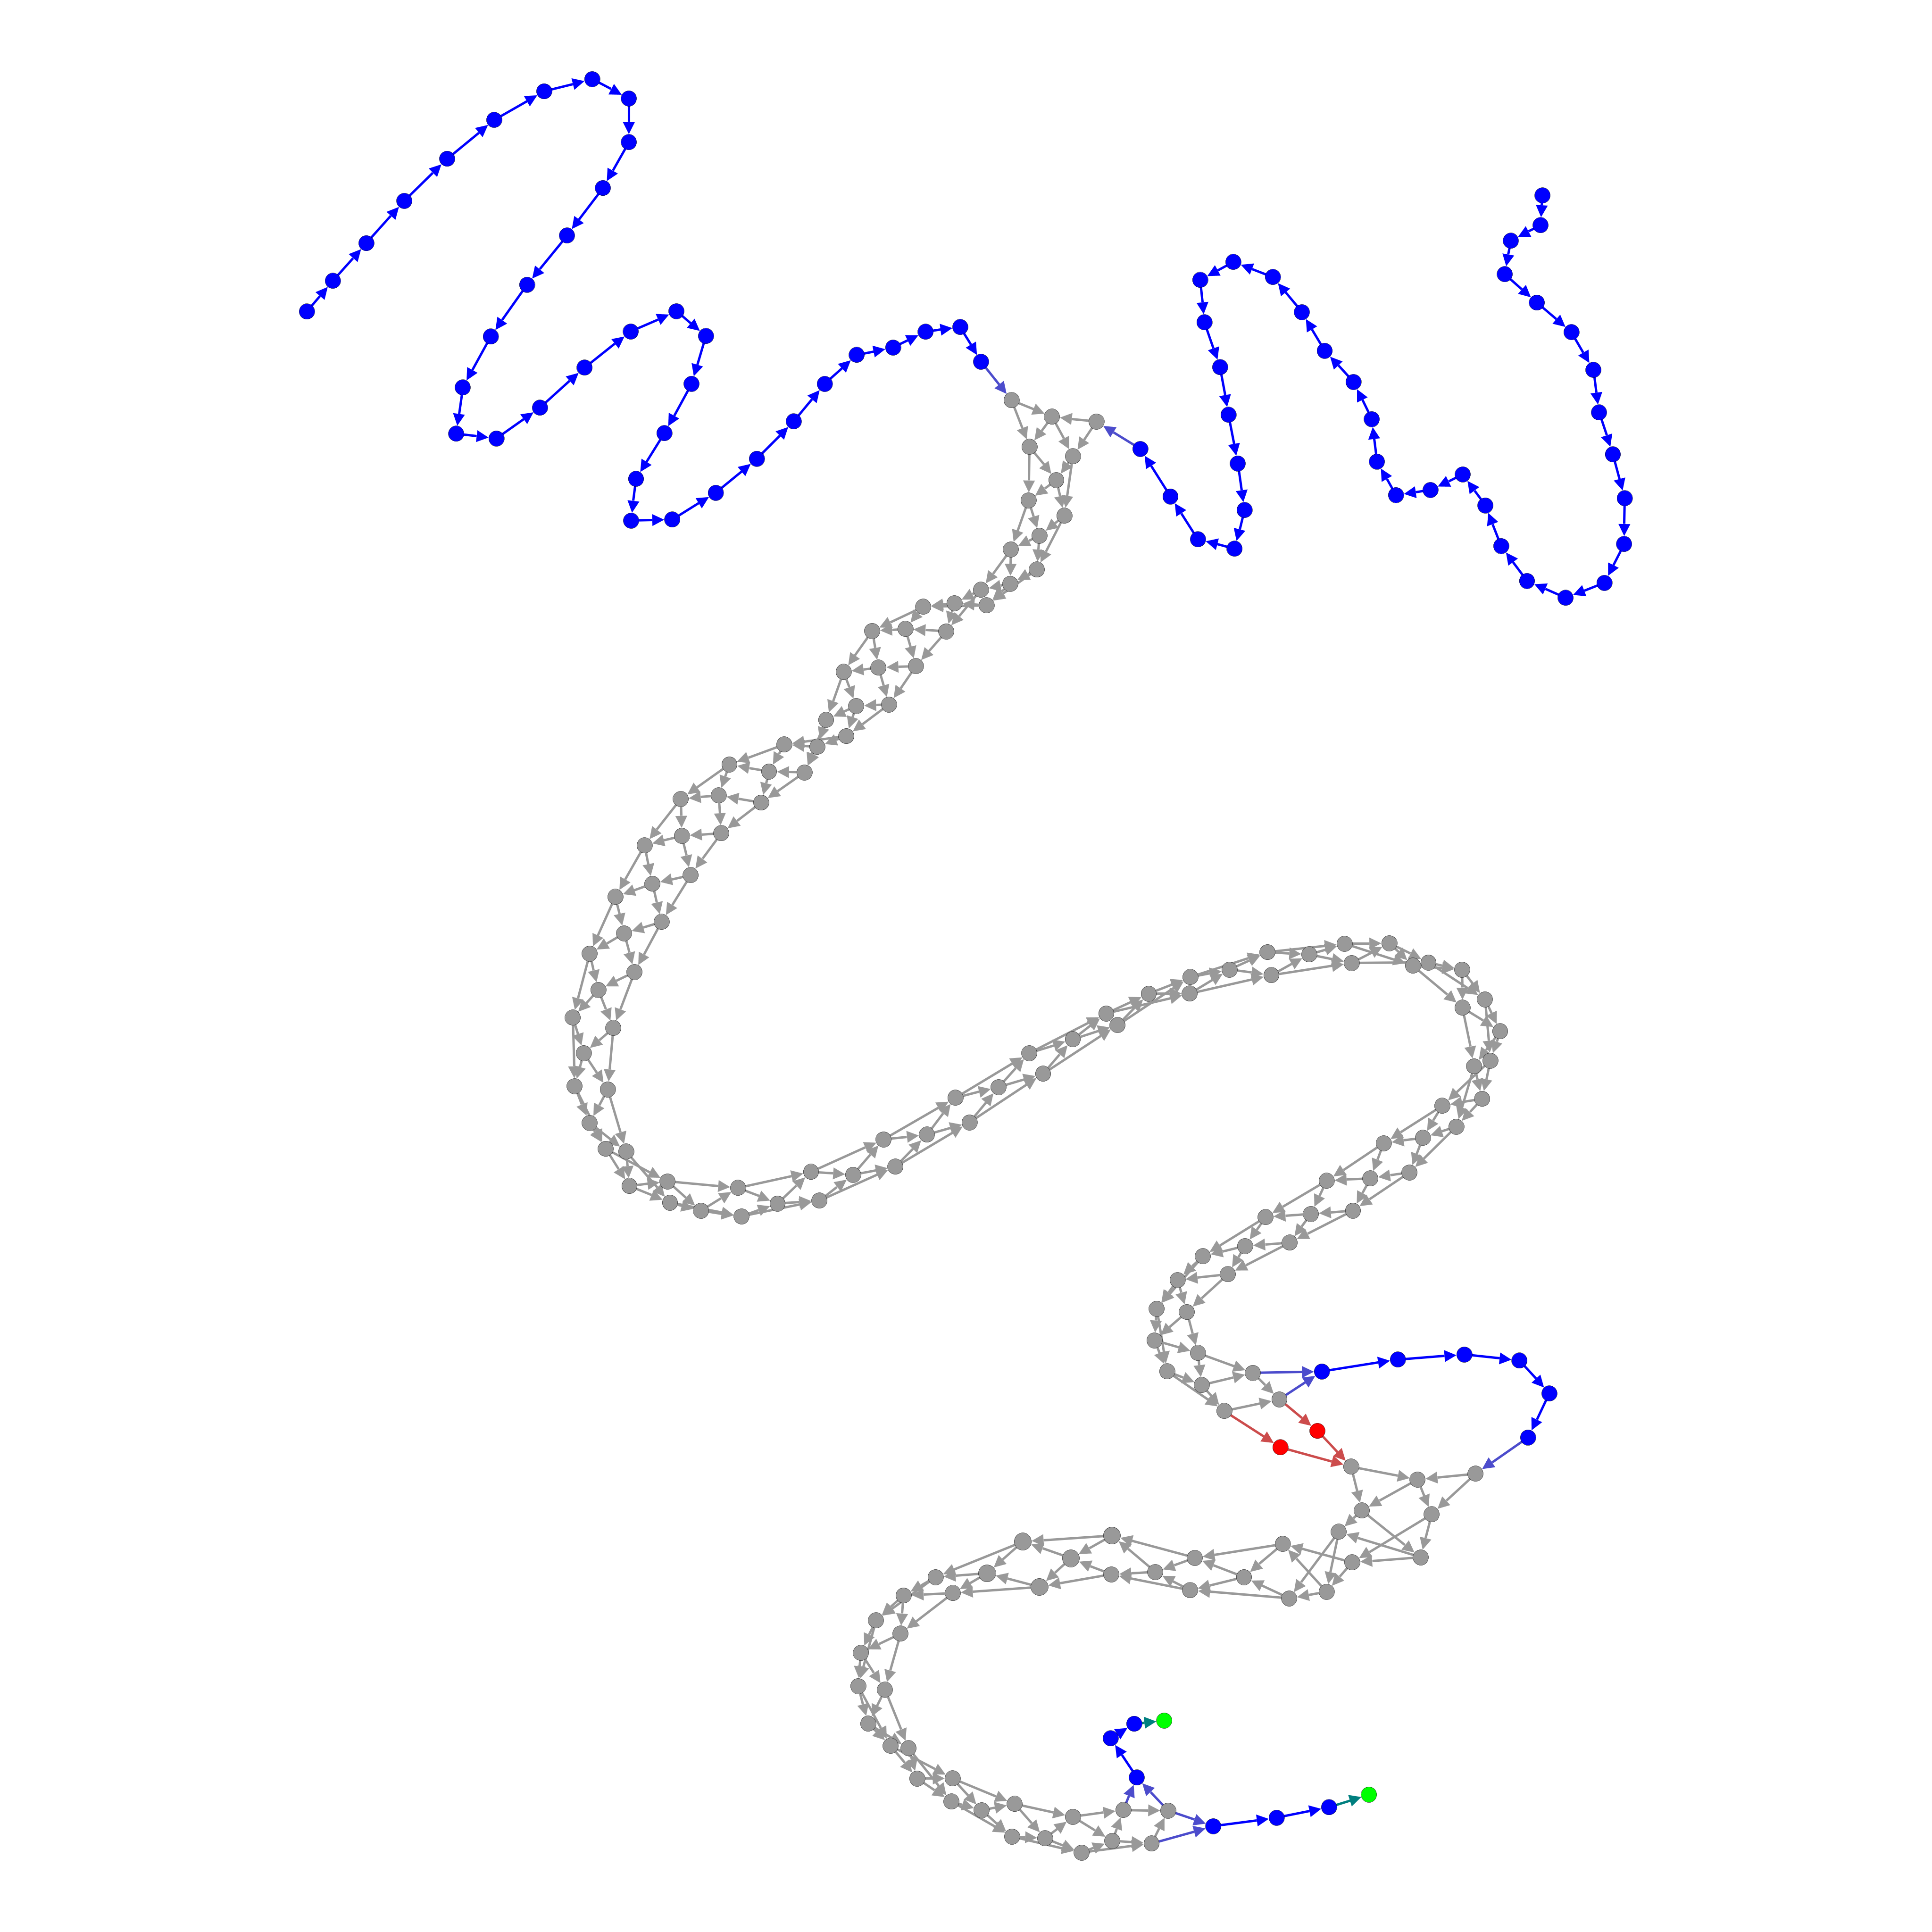
\includegraphics[scale=0.1]{experimentation/anonymous/anonymous.png}}
	\caption{MultiChain chain graph of a single download through 2 hops.}
	\label{fig:synthetic-anonymous-graph}
\end{figure}

The seeder and leecher both only interact with one hop.
These hops furthermore only interact with each other.
This can be clearly seen a part of the graph magnified in Figure \ref{fig:synthetic-anonymous-graph-magnified}.
The middle nodes represent the interaction between the hops.
The outer nodes are interactions between the seeder and the first hop and between the second hop and leecher.
The blocks are created alternating resulting in the graph pictured.

\begin{figure}
	\centerline{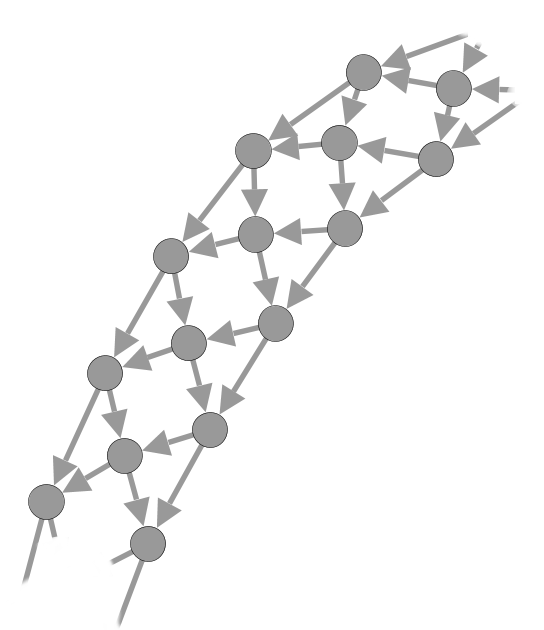
\includegraphics[scale=0.5]{experimentation/anonymous/anonymous-magnified.png}}
	\caption{Magnification of part of the graph.}
	\label{fig:synthetic-anonymous-graph-magnified}
\end{figure}

In the graph the timeout period can be seen clearly in Figure \ref{fig:synthetic-anonymous-graph}.
The two half-signed block can be seen in red.
The block with a reference coming from the outer block is the half-signed block belonging to the seeder.
The strain of blue nodes are the blocks created between the second hop and the leecher.
The red inner block is referenced by the first block created between the first hop and second hop after the timeout.






\subsection{Integrated anonymous download}
An substantial effort was made to integrated the tunnel community and hidden services community with the MultiChain community.
These communities work together to provide functionality to transfer data anonymously.
The tunnel community reports data transferred between peers and the MultiChain community add these amounts to the chain.
They are already integrated with BarterCast.
The method of integration of BarterCast was used to try to integrated MultiChain aswell.
Setting up the Gumby environment to run all communities took also considerable time.

Experiments were conducted where an 100 MB file is transferred by the actual anonymity communities,
while MultiChain transcribes the transfer amounts in the MultiChain.
The first experiment we ran was to test the integration without any hops.
In this setup the integration does not report any data transferred between the peers.
As such the scheduler never sees a reason to schedule a signature request.
The whole MultiChain community is never active.
MultiChain should also track these downloads,
but this requires MultiChain to be integrated in different places.

The second experiment was conducted with 2 hops.
The result of the experiment can be seen in Figure \ref{fig:integrated-anonymous-amounts}.
This shows that MultiChain does track the amount of upload and download for all peers in the network.
The hops roughly download and upload the same amount of their data.
This is what we expected as they just relay the data.
The seeder and downloader respectively only uploads and downloads.

Timeouts can be seen in the plots where the plot discontinues and does not grow steadily.
The reason these timeouts occur is that thresholds of the scheduler of every node is now reached at the same time resulting in a timeout.
Our recommendation is to have these thresholds to be shifted by a small amount randomly for every peer
to prevent them from overlapping.

\begin{figure}
\centering
\subfigure[Total download amount.]{
\centerline{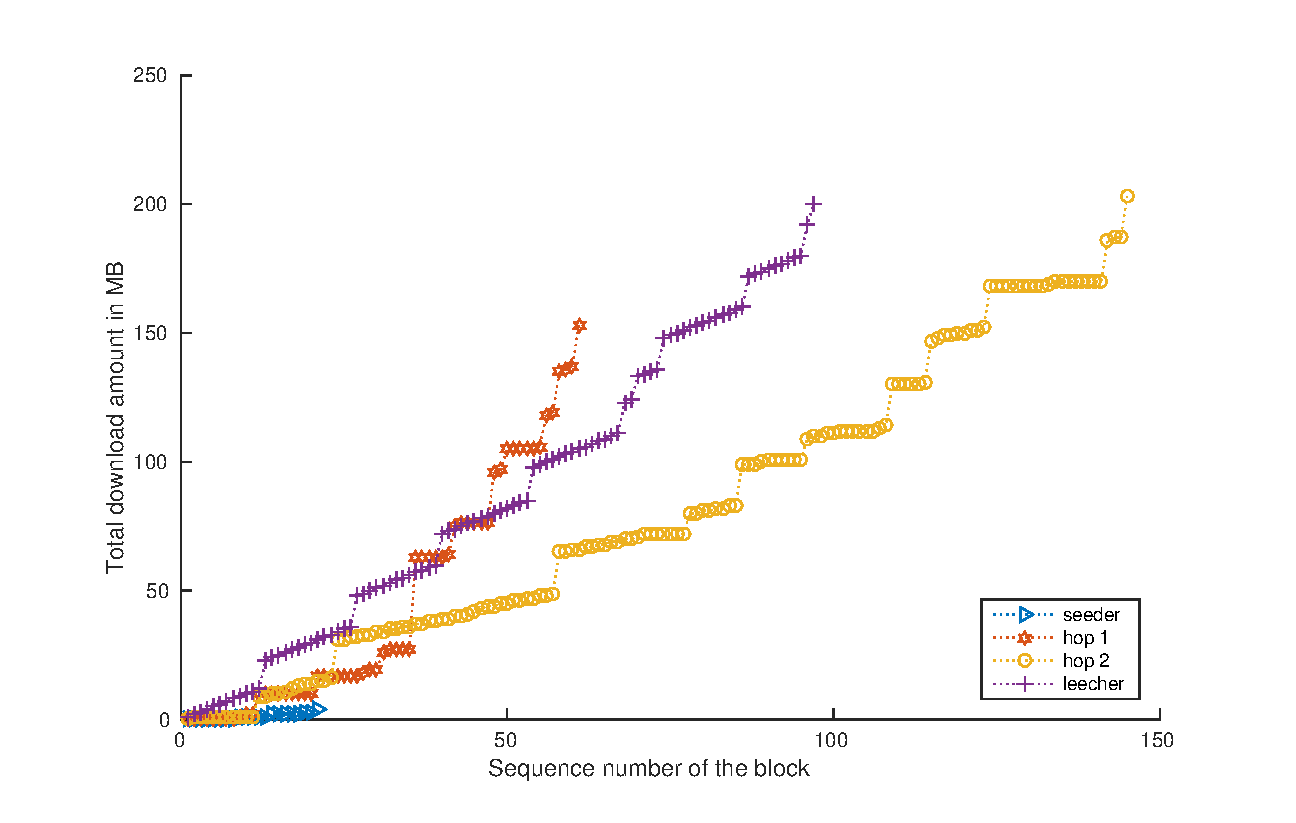
\includegraphics[scale=0.5]{experimentation/anonymous-integrated/integrated-anonymous-down.eps}}
\label{fig:integrated-anonymous-down}
}
\subfigure[Total upload amount.]{
\centerline{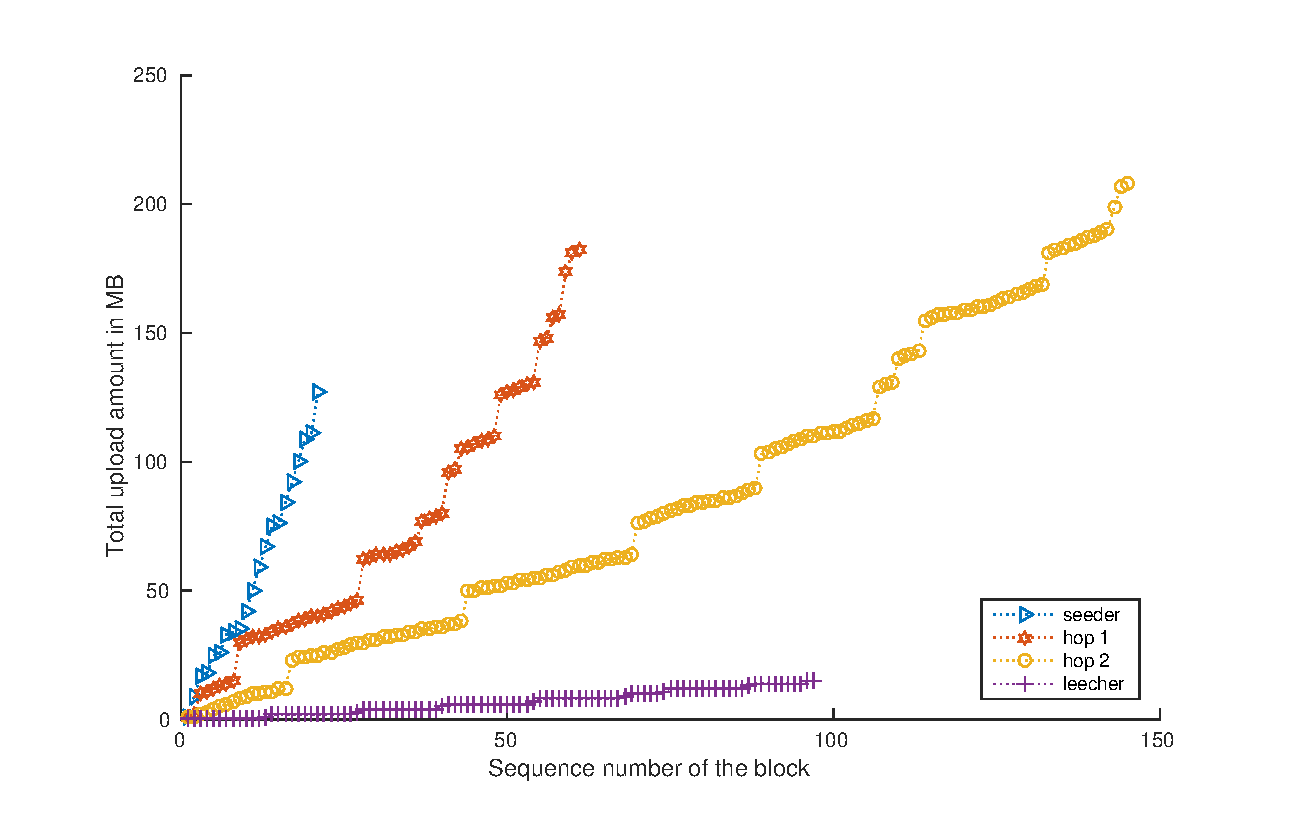
\includegraphics[scale=0.5]{experimentation/anonymous-integrated/integrated-anonymous-up.eps}}
\label{fig:integrated-anonymous-up}
}
\caption{Download and upload amounts during the integrated anonymous download experiment.}
\label{fig:integrated-anonymous-amounts}
\end{figure}

The amount of data that is reported to be transferred is remarkable.
The overhead measures twice the actual download size.
We therefore the conclusion that the integration is not properly and too much data is reported.
It is unclear where this data originates from.

Integrating MultiChain into the anonymous download communities is difficult,
because those communities do not use the standard classes used by Tribler to send messages.
These are necessary to properly integrate MultiChain and a complicated conversion was necessary.
Our recommendation is to refactor the anonymous download communities to use the standard classes
and to make it more clear in the code where data is sent and where data is received.
Also comments should be added to clarify the code.
Currently, there are no comments whatsoever.
This effort should atleast clarify why so much data is reported and will probaly fix the problem.

\section{Drop event recovery}
\label{sect:deadlock-exp}
MultiChain can run during normal operation into a situation
where a multiple of peers request to create blocks from each other as explained in section \ref{sect:deadlock}.
A specific experiment was conducted that created the situation manually.
This situation was also encountered during experimentation
and the experiment shows MultiChain correctly recovering from this situation.

\subsection{Forced drop event}
In this experiment a MultiChain node 1 tries to send a request to node 2 to create a block.
Node 2 is specifically configured for the purpose of the experiment
to ignore and drop all requests.
Node 1 now should wait for the response of the other node for a specific time.
During the time that node 1 is waiting a different request is sent from a normal node 3 to node 1.
This request will be dropped by node 1,
as it cannot process any incoming requests while node 1 has an outstanding request.
Node 1 and node 2 should timeout and continue operations.
After that node 2 will retransmit a request to node 1 and this should be completed correctly.

The experiment is locally run using gumby with all nodes running on a single computer.
Only three instances of MultiChain communities are started.
One of these instances never respond to a request to construct a block.
The logging of the every node is captured and recorded to verify the results of the experiment.

The output of the logging can be seen in Figure \ref{fig:manual-deadlock-experiment}.
First node 1 sends a signature request to node 2.
This message is ignored by node 2.
During the waiting period of node 1 a block request is sent to node 1 by node 3.
This request is also ignored, because node 1 cannot perform operations on the chain.
After the timeout period both node 1 and node 2 save an half-signed block to their chain
and can continue operations.
This is validated by a block created between node 3 and node 1.

\begin{figure}
\begin{FVerbatim}[fontsize=\small]
1: Requesting Signature for candidate: 2
1: Chain Exclusion: signature request: False
1: Chain Exclusion: acquired, sending signature request.
1: Sending signature request.
2: Received signature request that will be ignored.

3: Requesting Signature for candidate: 1
3: Chain Exclusion: signature request: False
3: Chain Exclusion: acquired, sending signature request.
3: Sending signature request.
1: Received signature request.
1: Chain Exclusion: process request: True
1: Chain Exclusion: not acquired. Dropping request.

1: Timeout received for signature request.
1: Persisting sr: bFOXhHT2ffSrtIn9tuMfEGGarGY=
3: Timeout received for signature request.
3: Persisting sr: l1O8UquXdxWdkg+KAYZ1FYocwjo=
3: Requesting Signature for candidate: 1

3: Chain Exclusion: signature request: False
3: Chain Exclusion: acquired, sending signature request.
3: Sending signature request.
1: Received signature request.
1: Chain Exclusion: process request: False
1: Chain Exclusion: acquired to process request.
1: Persisting sr: 7Y86Ck4duwTduP6j/aIRrWHAZqw=
1: Sending signature response.
3: Signature response received. Modified: True
3: Valid 1 signature response(s) received.
3: Persisting sr: 7Y86Ck4duwTduP6j/aIRrWHAZqw=
3: Chain exclusion: released received signature response.
\end{FVerbatim}
    \caption{Output of the manual drop event experiment}~\label{fig:manual-deadlock-experiment}
\end{figure}

\subsection{Naturally occuring drop events}
In the experiment a 100 megabyte file was downloaded anonymously with 2 hops.
Anonymously downloading is described more in the thesis report of R. Ruigrok~\cite{ruigrok-anonymous}.
There are 2 Triblers instances with exit functionality and 18 instances without exit functionality.
All instances are run locally on one machine.
The instances are run in parallel,
so the fact that all instances are run on a single machine does not cause the drop event to occur.
There is no packetloss in this experiment.
The corresponding graph of all the MultiChains of the experiment can be seen in Figure \ref{fig:deadlock-double}.

The potential scenario of two peers both waiting can be seen multiple times in the graph and are encircled.
The scenario generates a half-signed block at both peers.
Usually the peers continue collaboration and this continuation of a sequence can be seen in subsequent blocks.
In the graph a more complicated scenario can also be seen where multiple peers timeout between each other.
The graph shows that MultiChain correctly recovers from all scenario's.

\begin{figure}
	\centerline{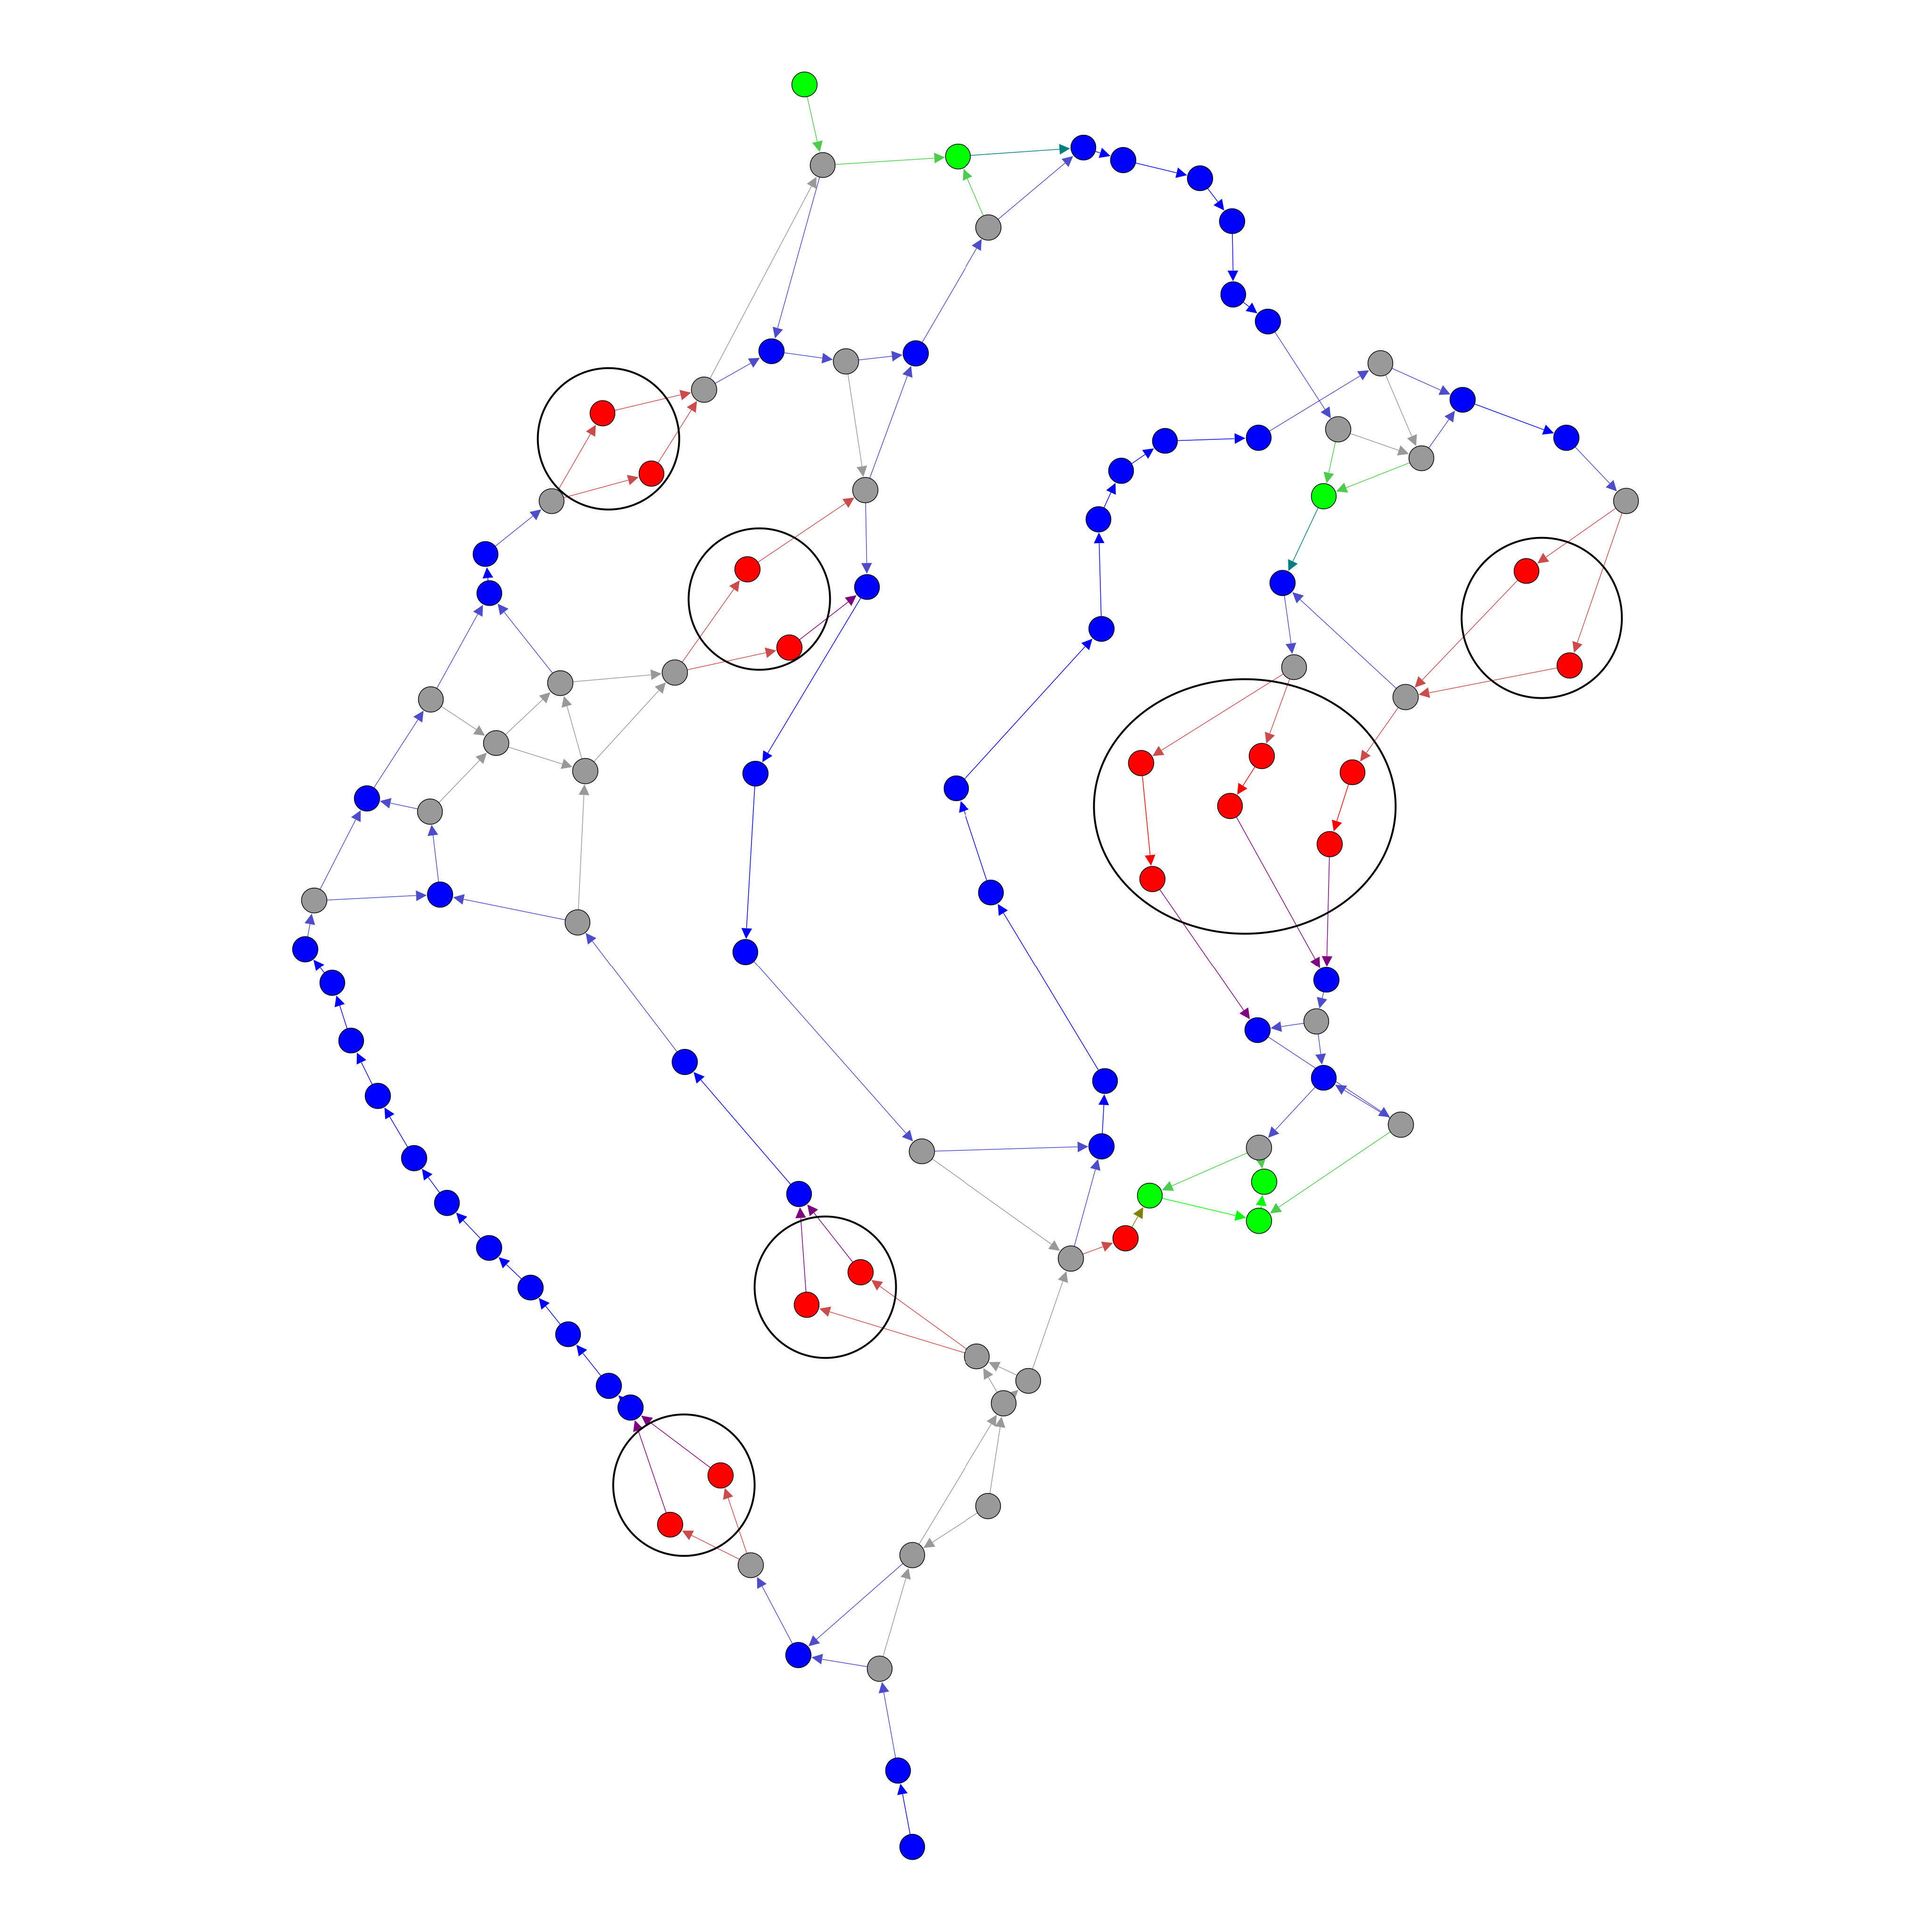
\includegraphics[scale=0.1]{experimentation/deadlock/deadlock.png}}
	\caption{Mixing of double-signed blocks(blue/grey) and half-signed blocks(red) in MultiChain.}
	\label{fig:deadlock-double}
\end{figure}


%Problems
\chapter{Known vulnerabilities}
\label{problems}
There are several known security vulnerabilities with the current design.
As said in section \ref{pb-aim} an incremental approach was taken.
As such, the design is part of a bigger system that as a whole is to be deployed in the real world.
In this section we will describe the known vulnerabilities
and explain the future work that is needed to solve these.

\section{Branch attack}
In this section we will explain an attack that can be done by a malicious node M.
The attack consists of obscuring a part of his transaction history.
M creates a new branch of his transaction history that is more favourable to him.

\subsection{Abandoning full transaction history distribution}
One of the main pillars of the design is to not distribute
and have one common, full transaction history between every peer.
While this is the main pillar of design for the blockchain of Bitcoins.
The reasoning behind the idea to abandon is that a common, full truth
will limit the amount of interactions that can be processed
or the participiation of less powerfull machines.

The reason for the limitation is that every interactions will have to be distributed to every peer in the network.
Every transaction has to be processed by every node at the cost of bandwidth, compute power and storage.
The cost might be very limited for a single transaction,
but with greater scale these cost will add up.
The amount of these three resources is limited and will limit the amount of transactions that can be processed.

The limitation can be delayed by naturally excluding participation of less powerfull devices.
For example, mobile devices have generally much less storage available.
When the full transaction history becomes too large,
participation of these mobile devices is excluded due to the fact that they cannot fully store the transaction history.
This problem can be seen to affect Bitcoins and has been demonstrated in section \ref{bitcoin-limit-size}.

\subsection{Alternating partial transaction history}
A malicious node M has his own chain of transactions
and he wants to falsify his transactions after a certain point.
He wants to rewrite his transaction history from that point and create an alternate transaction history.
M wants to do this to whitewash his reputation.
The node can simply choose to forget and obscure blocks after that point.
A new branch will be created by chaining new blocks to the desired point in history.

\begin{figure}
	\centerline{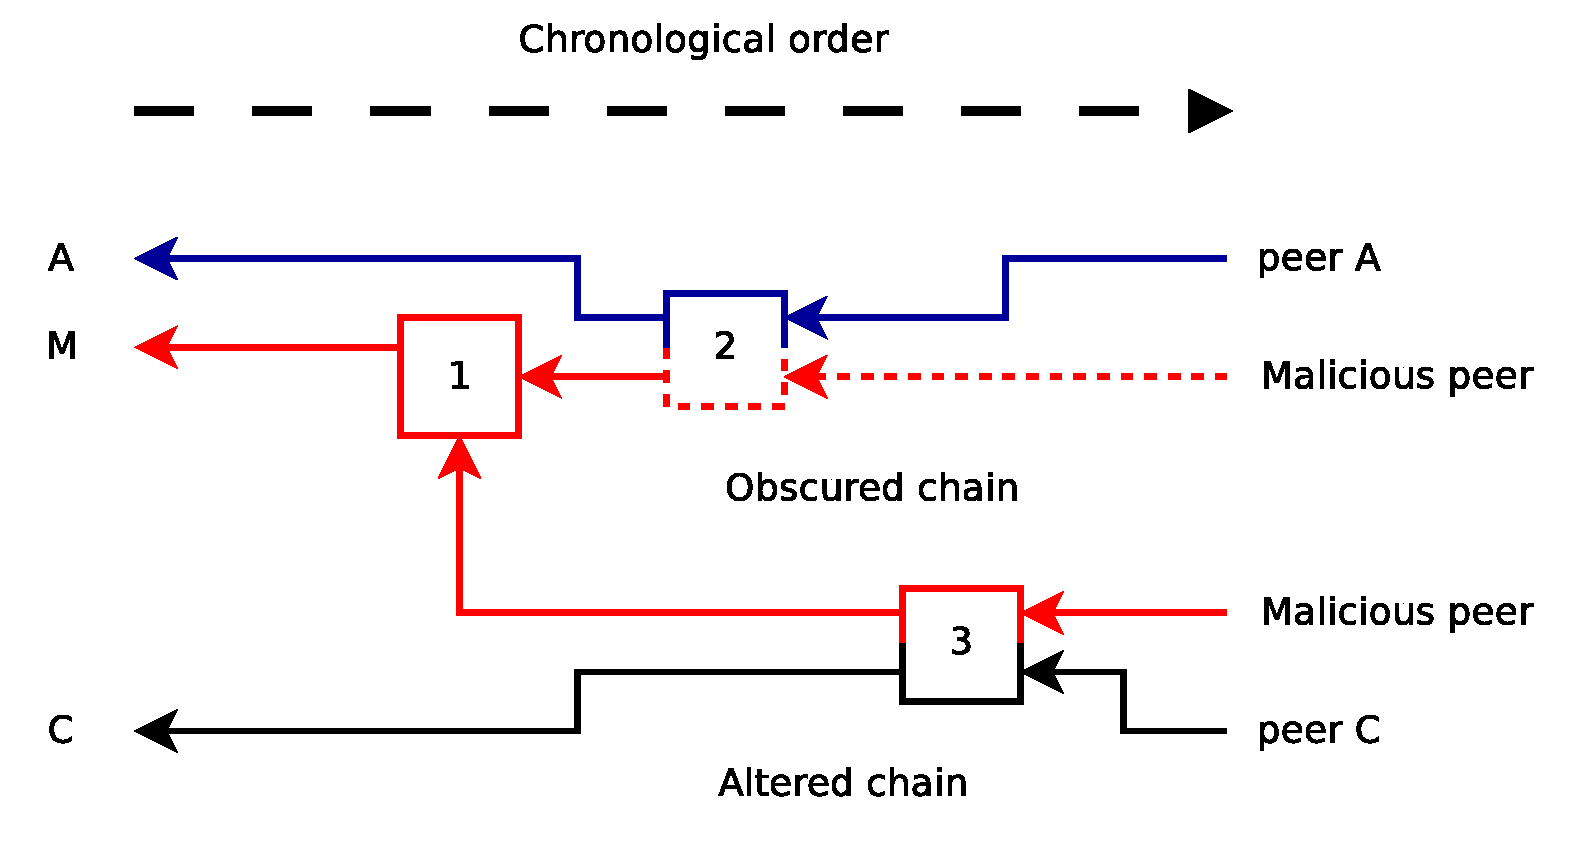
\includegraphics[scale=0.3]{problems/figs/branch.eps}}
	\caption{Example of a branch created by M.}
	\label{fig:problem-branch-obscure}
\end{figure}

In Figure \ref{fig:problem-branch-obscure} an example can be seen of a branch created by M.
In this example M tries to obscure block 2 and any subsequent blocks from C.
When C requests the transaction history of M, M will only send the transaction history up to block 1.
When M and C create a block together,
M will reuse the hash of block 1 in the new block.
For clarity of the diagram, the node interacting with M in block 1 is not displayed.

Now malicious node M does have the problem that not only he knows his transaction history.
When M interacted with node A a block was created that M tries to obscure.
A has this block in his own chain
and therefore knows about it being part of the transaction history of M.
This can be seen in the example in Figure \ref{fig:problem-branch-obscure}.

M will want to reduce the likelyhood of the detection of his fraud.
If his fraud is detected, he might be punished and no longer to continue his abuse.
The first way to minimize detection is to choose
to only interact with new nodes that do not know about the alternate part of the transaction history.
Nodes that have requested an alternate part of the transaction history
or that have been interacted directly with are no longer interacted with.
In a sufficiently healthy network this will result in node M being able to find new nodes to help him.

\begin{figure}
	\centerline{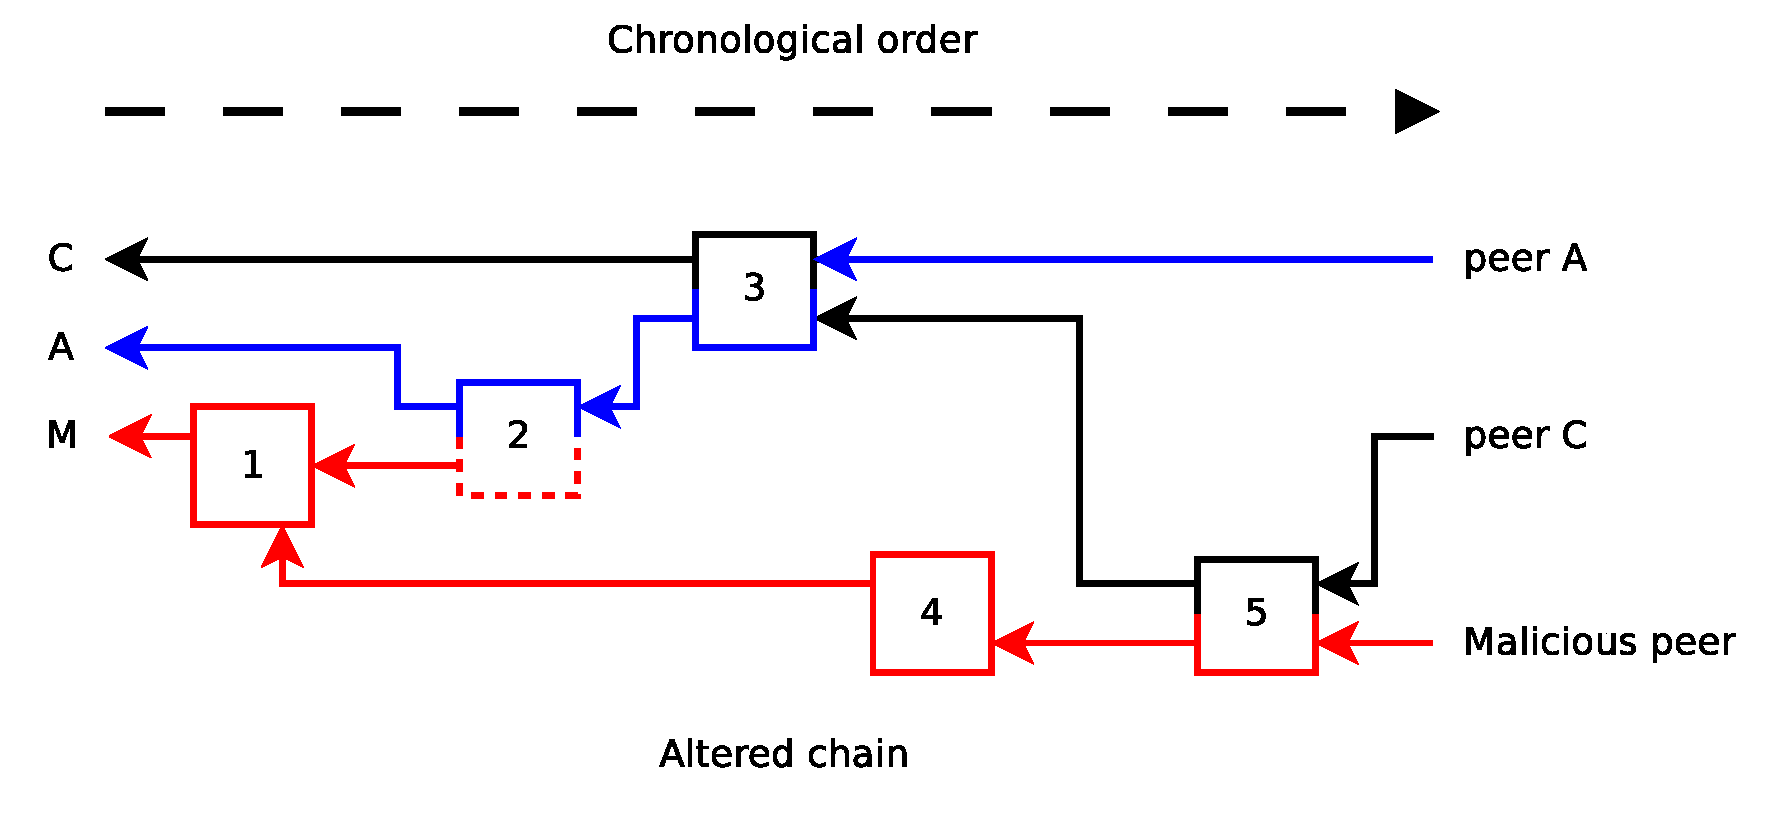
\includegraphics[scale=0.3]{problems/figs/branch-fraud-detected.eps}}
	\caption{Detectable fraud by C.}
	\label{fig:problem-branch-preknowledge}
\end{figure}

There is another example that will expose the fraud of M.
This example can be seen in Figure \ref{fig:problem-branch-preknowledge}.
A node C might still exposes the cheating of M by chance.
C can have an interaction with node A by coincidence.
Before creating block 3 C will request the transaction history of node A containing an obscured block of M.
Now when M wants to interact with C, M will want to create block 5.
When C requests the full transaction history of M, it will detect that the transaction history of M no longer contains block 2.
This exposes the fraud of M.

But C will have no sure way of exposing this type of fraud by his own doing,
except for requesting every transaction history of every node in the system.
This is in a way a common, full transaction history and was chosen to be avoided by the design to become more scalable.
C can limited the possibility of the attack by increasing his knowledge by collecting more transaction history of other nodes.
If node A or B stop participating and exit the network,
then C will have no way of detecting the fraud by M.

The second way M can limit the exposure of his cheating is in a more sophisticated way.
He can present several, different transaction history to different nodes.
M will continue keeping track of the unmodified transaction history.
When M wants to interact with A or B, both knowing this transaction history, he will present this transaction history.
So M can still interact with A and B.
But when interacting with C he will present his alternate transaction history.
C will only expose the fraud in the same way as previously.

\subsection{Possibility of attack and likelyhood of detecting fraud}
This attack can always be done M and is not limited to circumstances.
Also the attack is not limited and M can try to fool any number of other nodes C.
As shown in Figure \ref{fig:branch-multiple}.

\begin{figure}
	\centerline{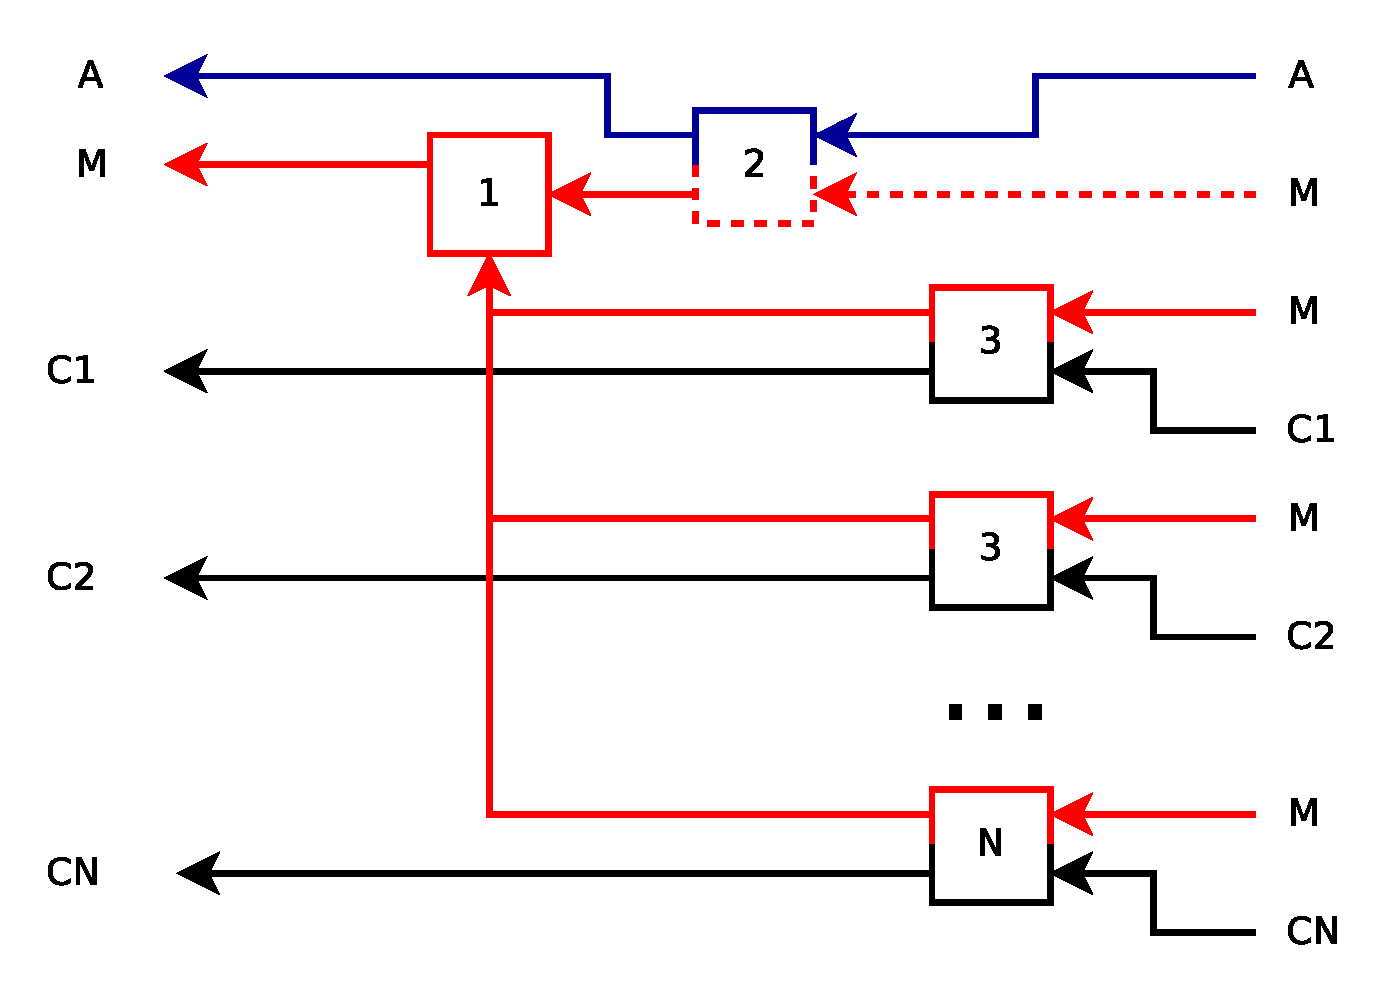
\includegraphics[scale=0.3]{problems/figs/branch-multiple.eps}}
	\caption{Example of multiple branches created by M.}
	\label{fig:branch-multiple}
\end{figure}



The likelyhood of exposing this attack depends on several factors
and will be the only factor to limit M in performing this fraud.
The likelihood depends on:
\begin{itemize}
\item Size of the network
\item Likelihood of interactions between A or B and C
\end{itemize}

All these properties will influence the chance of C coming across an obscured block.

\subsection{Possible punishment of this attack}
When the fraud is detected C can only punish M by no longer interacting with him.
There is currently no way of making it globally know to every node in the network that fraud was committed.
So only M is punished by C and can continue his abuse of other nodes in the network.
It is recommended as future work to do so.

\section{The Sybil Attack}

In this section we will explain the Sybil Attack\cite{douceur-sybil}
and how it can be used in the MultiChain system to create an artificial reputation.
An universallly applicable solution has not yet be found\cite{levine-sybilsurvey}.

\subsection{Using fake indentities}
In large distributed systems convincingly distinct identities can be presented
that are infact all under the control of a single adversary M.
Identities can be public keys like in the Dispersy system
or other abstractions of information without direct physical knowledge.
These identities can participate in the system acting like normal agents,
but they can also help each other malificiently to boost each other towards a common goal.

In the MultiChain system the attack is done in the following way.
M creates several other identities besides his own.
This involves generating several key pairs.
Now M controls several identities that can be presented convincingly.
The key pairs do not have to be linked to a node responding to requests.
Failure of nodes are typical in large distributed systems.

Using these key pairs M can now generate an artificial reputation.
Transactions between M and the fake identities are generated by M.
These are signed using the keys of the fake identities.
Using a single transaction it cannot be determined if it is between two distinct identities or a single distinct identity and a fake identity.

\begin{figure}
	\centerline{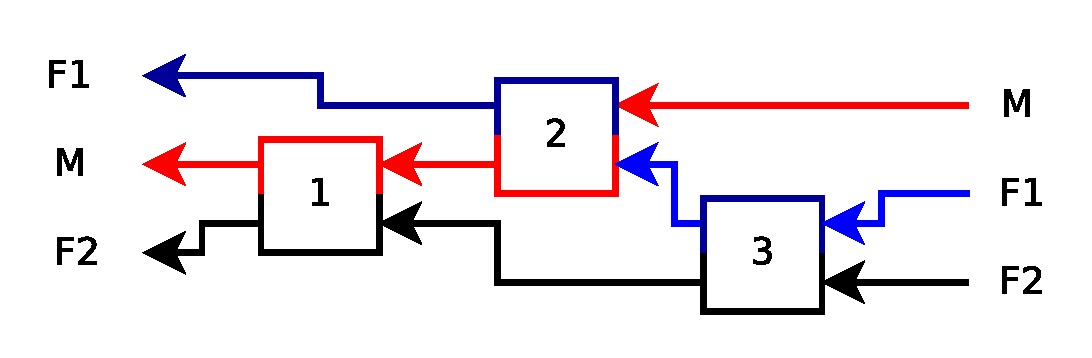
\includegraphics[scale=0.3]{problems/figs/sybil.eps}}
	\caption{The sybil attack by M.}
	\label{fig:sybil-example}
\end{figure}

An example of the Sybil Attack can be seen in \ref{fig:sybil-example}.
In this example M is the malificient node and F1 and F2 his fake identities.
Block 1 and block 2 contain a transaction that is favourable to M,
but M has done nothing to deserve these.
Similair blocks like block 3 can be generated between fake identities in an effort to thwart efforts to analyse the network
and detect fake identities.

In this way M is able to boost his reputation without much work.
The more sophisticated the generation is done by M,
the harder it will be to detect that M boosted his reputation using fake identities.
M can then abuse his fake reputation by solliciting cooperation from other nodes in the network.
They will respond positively on the request by M based upon the false reputation M claims to have.

\subsection{Validating Identities}
A node can have three potential sources of validation of distinct identities:
\begin{itemize}
\item Itself
\item Other entitites
\item A trusted, central authority
\end{itemize}

A node itself could try to directly validate two identities to be distinct.
It would challenge several identities to complete a task that only two entities could complete.
The task would require more resources then a single entity possesses and will be issued simultaneously to all identities.
If the identities complete the task, they have proven to be distinct.
Example of required resources are communication, storage and computation.
These challenges can scale to validate more entities at once.

Indirect validation can be used by a node to by delegating validation to other entities.
A node could accept additional identities to be distinct when an accepted identity vouches for it.
The node has the delegated responsibility to challenge the entity with a challenge.
This would limit the total amount of challenges needed.
But an obvious pitfall of delegating this to other identities is that these can vouch for fraudelent identities.
Next to this, it involves an increase in complexity as the challenges still have to be issued concurrently.

But these challenges are highly indesirable.
These challenges require by definition to occupy between two nodes a limited resource to the maximum capacity of a single node.
While not providing any additional functionality beyond asserting distinct identities.
These challenges also prove inworkable when entities have hugely different amount of resources available.
No challenge can be constructed that can be worked by less powerfull devices,
that could not be worked several times by more powerfull devices.

Next to this, these challenges are only usable with nodes that are active and responding to challenges.
If a node becomes inactive it cannot be ascertained if the node is a fake identity.
But this identity still makes claim about a reputation of another entity.
A choice has to be made between either not counting these claims and allow for a drop in reputation of a node or
allow claims that cannot be validated to be taken into account.
Both options lower the usability of the system.

A trusted, central authority would be able to vouch for distinct indentities
if it has an other way outside the system of asserting that it indeed is a distinct identity.
Approaches exists that implicitly rely on the authority of a trusted agency.
But a central authority goes against the principles of a peer-to-peer network.

Several other defenses against the Sybil Attack have been proposed\cite{newsome-sybil}\cite{dinger-sybil}
or variants on the defenses stated here\cite{levine-sybilsurvey}.
But these either have the same limitation and are minor improvements or are non-applicable for MultiChain.

\subsection{Possibility of attack and likelyhood of detecting fraud}
For M to conduct the Sybil Attack he will need to generate a set of key pairs.
This is trivial to do and Dispersy provides functionality to do this very easily.

%TODO Timing of generating several keys

With these keys M has to generate blocks.

%TODO timing of generating blocks

Sybil Attack can have a wide range of sophistication.
Ranging from a large amount of fake identities with a large amount of transaction between them
to a single, fake identity boosting the reputation of M in a couple of transaction.
Even these simple Sybil Attack are hard to defend against if these are not done to obviously.




%Conclusion
\chapter{Conclusion}

% BIBLIOGRAPHY
\bibliographystyle{bib/latex8}
\bibliography{bib/bibliography}

%\appendix

%\include{appendix_a}

\end{document}

